\ifdefined\included
\else
\documentclass[a4paper,11pt,twoside]{StyleThese}
\usepackage{amsmath,amssymb, amsthm}             % AMS Math
\usepackage[T1]{fontenc}
\usepackage[utf8x]{inputenc}
\usepackage{babel}
\usepackage{datetime}

\usepackage{silence}

\WarningFilter{minitoc(hints)}{W0023}
\WarningFilter{minitoc(hints)}{W0028}
\WarningFilter{minitoc(hints)}{W0030}

\usepackage{lmodern}
\usepackage{tabularx}
%\usepackage{tabular}
\usepackage{multirow}
\usepackage{xspace}

\usepackage{subfig}
\usepackage[inline]{enumitem}

\usepackage{hhline}
\usepackage[left=1.5in,right=1.3in,top=1.1in,bottom=1.1in,includefoot,includehead,headheight=13.6pt]{geometry}
\renewcommand{\baselinestretch}{1.05}

% Table of contents for each chapter

\usepackage[nottoc, notlof, notlot]{tocbibind}
\usepackage{minitoc}
\setcounter{minitocdepth}{2}
\mtcindent=15pt
% Use \minitoc where to put a table of contents

\usepackage{aecompl}

% Glossary / list of abbreviations

\usepackage[intoc]{nomencl}
\iftoggle{ThesisInEnglish}{%
\renewcommand{\nomname}{Glossary}
}{ %
\renewcommand{\nomname}{Liste des Abréviations}
}

\usepackage{etoolbox}
\renewcommand\nomgroup[1]{%
  \item[\bfseries
  \ifstrequal{#1}{A}{Number Sets}{%
  \ifstrequal{#1}{G}{Agents Beliefs and Action Models}{%
  \ifstrequal{#1}{N}{Navigation}{%
  \ifstrequal{#1}{O}{Ontology}{%
  \ifstrequal{#1}{R}{Referring Expression Generation}{%
  \ifstrequal{#1}{Z}{Controllable and Uncontrollable Agents Task Planning}{}}}}}}%
]}

\makenomenclature



% My pdf code

\usepackage{ifpdf}

\ifpdf
  \usepackage[pdftex]{graphicx}
  \DeclareGraphicsExtensions{.jpg}
  \usepackage[pagebackref,hyperindex=true]{hyperref}
  \usepackage{tikz}
  \usetikzlibrary{arrows,shapes,calc}
\else
  \usepackage{graphicx}
  \DeclareGraphicsExtensions{.ps,.eps}
  \usepackage[dvipdfm,pagebackref,hyperindex=true]{hyperref}
\fi

\graphicspath{{.}{images/}}

%% nicer backref links. NOTE: The flag ThesisInEnglish is used to define the
% language in the back references. Read more about it in These.tex

\iftoggle{ThesisInEnglish}{%
\renewcommand*{\backref}[1]{}
\renewcommand*{\backrefalt}[4]{%
\ifcase #1 %
(Not cited.)%
\or
(Cited in page~#2.)%
\else
(Cited in pages~#2.)%
\fi}
\renewcommand*{\backrefsep}{, }
\renewcommand*{\backreftwosep}{ and~}
\renewcommand*{\backreflastsep}{ and~}
}{%
\renewcommand*{\backref}[1]{}
\renewcommand*{\backrefalt}[4]{%
\ifcase #1 %
(Non cité.)%
\or
(Cité en page~#2.)%
\else
(Cité en pages~#2.)%
\fi}
\renewcommand*{\backrefsep}{, }
\renewcommand*{\backreftwosep}{ et~}
\renewcommand*{\backreflastsep}{ et~}
}

% Links in pdf
\usepackage{color}
\definecolor{linkcol}{rgb}{0,0,0.4} 
\definecolor{citecol}{rgb}{0.5,0,0} 
\definecolor{linkcol}{rgb}{0,0,0} 
\definecolor{citecol}{rgb}{0,0,0}
% Change this to change the informations included in the pdf file

\hypersetup
{
bookmarksopen=true,
pdftitle="Endowing the robot with the abilities to control and evaluate its contribution to a human-robot joint action",
pdfauthor="Amandine MAYIMA", %auteur du document
pdfsubject="Thèse", %sujet du document
%pdftoolbar=false, %barre d'outils non visible
pdfmenubar=true, %barre de menu visible
pdfhighlight=/O, %effet d'un clic sur un lien hypertexte
colorlinks=true, %couleurs sur les liens hypertextes
pdfpagemode=None, %aucun mode de page
pdfpagelayout=SinglePage, %ouverture en simple page
pdffitwindow=true, %pages ouvertes entierement dans toute la fenetre
linkcolor=linkcol, %couleur des liens hypertextes internes
citecolor=citecol, %couleur des liens pour les citations
urlcolor=linkcol %couleur des liens pour les url
}

% definitions.
% -------------------

\setcounter{secnumdepth}{3}
\setcounter{tocdepth}{2}

% Some useful commands and shortcut for maths:  partial derivative and stuff

\newcommand{\pd}[2]{\frac{\partial #1}{\partial #2}}
\def\abs{\operatorname{abs}}
\def\argmax{\operatornamewithlimits{arg\,max}}
\def\argmin{\operatornamewithlimits{arg\,min}}
\def\diag{\operatorname{Diag}}
\newcommand{\eqRef}[1]{(\ref{#1})}

\usepackage{rotating}                    % Sideways of figures & tables
%\usepackage{bibunits}
%\usepackage[sectionbib]{chapterbib}          % Cross-reference package (Natural BiB)
%\usepackage{natbib}                  % Put References at the end of each chapter
                                         % Do not put 'sectionbib' option here.
                                         % Sectionbib option in 'natbib' will do.
\usepackage{fancyhdr}                    % Fancy Header and Footer

% \usepackage{txfonts}                     % Public Times New Roman text & math font
  
%%% Fancy Header %%%%%%%%%%%%%%%%%%%%%%%%%%%%%%%%%%%%%%%%%%%%%%%%%%%%%%%%%%%%%%%%%%
% Fancy Header Style Options

\pagestyle{fancy}                       % Sets fancy header and footer
\fancyfoot{}                            % Delete current footer settings

%\renewcommand{\chaptermark}[1]{         % Lower Case Chapter marker style
%  \markboth{\chaptername\ \thechapter.\ #1}}{}} %

%\renewcommand{\sectionmark}[1]{         % Lower case Section marker style
%  \markright{\thesection.\ #1}}         %

\fancyhead[LE,RO]{\bfseries\thepage}    % Page number (boldface) in left on even
% pages and right on odd pages
\fancyhead[RE]{\bfseries\nouppercase{\leftmark}}      % Chapter in the right on even pages
\fancyhead[LO]{\bfseries\nouppercase{\rightmark}}     % Section in the left on odd pages

\let\headruleORIG\headrule
\renewcommand{\headrule}{\color{black} \headruleORIG}
\renewcommand{\headrulewidth}{1.0pt}
\usepackage{colortbl}
\arrayrulecolor{black}

\fancypagestyle{plain}{
  \fancyhead{}
  \fancyfoot{}
  \renewcommand{\headrulewidth}{0pt}
}

%\usepackage{MyAlgorithm}
%\usepackage[noend]{MyAlgorithmic}
\usepackage{algorithm}
\usepackage[noend]{algpseudocode}
\usepackage{comment}
\usepackage[ED=MITT-InfoTel, Ets=INSA]{tlsflyleaf}
%%% Clear Header %%%%%%%%%%%%%%%%%%%%%%%%%%%%%%%%%%%%%%%%%%%%%%%%%%%%%%%%%%%%%%%%%%
% Clear Header Style on the Last Empty Odd pages
\makeatletter

\def\cleardoublepage{\clearpage\if@twoside \ifodd\c@page\else%
  \hbox{}%
  \thispagestyle{empty}%              % Empty header styles
  \newpage%
  \if@twocolumn\hbox{}\newpage\fi\fi\fi}

\newcommand*{\algrule}[1][\algorithmicindent]{%
	\makebox[#1][l]{%
		\hspace*{.2em}% <------------- This is where the rule starts from
		\vrule height .75\baselineskip depth .25\baselineskip
	}
}

%%% to have lines in algorithm, from stackexchange
\newcount\ALG@printindent@tempcnta
\def\ALG@printindent{%
	\ifnum \theALG@nested>0% is there anything to print
	\ifx\ALG@text\ALG@x@notext% is this an end group without any text?
	% do nothing
	\else
	\unskip
	% draw a rule for each indent level
	\ALG@printindent@tempcnta=1
	\loop
	\algrule[\csname ALG@ind@\the\ALG@printindent@tempcnta\endcsname]%
	\advance \ALG@printindent@tempcnta 1
	\ifnum \ALG@printindent@tempcnta<\numexpr\theALG@nested+1\relax
	\repeat
	\fi
	\fi
}
% the following line injects our new indent handling code in place of the default spacing
\patchcmd{\ALG@doentity}{\noindent\hskip\ALG@tlm}{\ALG@printindent}{}{\errmessage{failed to patch}}
\patchcmd{\ALG@doentity}{\item[]\nointerlineskip}{}{}{} % no spurious vertical space
% end vertical rule patch for algorithmicx

\makeatother
 
%%%%%%%%%%%%%%%%%%%%%%%%%%%%%%%%%%%%%%%%%%%%%%%%%%%%%%%%%%%%%%%%%%%%%%%%%%%%%%% 
% Prints your review date and 'Draft Version' (From Josullvn, CS, CMU)
\newcommand{\reviewtimetoday}[2]{\special{!userdict begin
    /bop-hook{gsave 20 710 translate 45 rotate 0.8 setgray
      /Times-Roman findfont 12 scalefont setfont 0 0   moveto (#1) show
      0 -12 moveto (#2) show grestore}def end}}
% You can turn on or off this option.
% \reviewtimetoday{\today}{Draft Version}
%%%%%%%%%%%%%%%%%%%%%%%%%%%%%%%%%%%%%%%%%%%%%%%%%%%%%%%%%%%%%%%%%%%%%%%%%%%%%%% 

\newenvironment{maxime}[1]
{
\vspace*{0cm}
\hfill
\begin{minipage}{0.5\textwidth}%
%\rule[0.5ex]{\textwidth}{0.1mm}\\%
\hrulefill $\:$ {\bf #1}\\
%\vspace*{-0.25cm}
\it 
}%
{%

\hrulefill
\vspace*{0.5cm}%
\end{minipage}
}

\let\minitocORIG\minitoc
\renewcommand{\minitoc}{\minitocORIG \vspace{1.5em}}

\usepackage{multirow}
%\usepackage{slashbox}

\newenvironment{bulletList}%
{ \begin{list}%
	{\tiny$\bullet$}%
	{\setlength{\labelwidth}{25pt}%
	 \setlength{\leftmargin}{30pt}%
	 \setlength{\itemsep}{-0.5em}}}%
{ \end{list} }

\newenvironment{inlineEnumerate}
{\begin{enumerate*} [label={(\arabic*)}] }
{\end{enumerate*}}

\theoremstyle{definition}
\newtheorem{definition}{Definition}
\renewcommand{\epsilon}{\varepsilon}

% centered page environment

\newenvironment{vcenterpage}
{\newpage\vspace*{\fill}\thispagestyle{empty}\renewcommand{\headrulewidth}{0pt}}
{\vspace*{\fill}}

\newenvironment{asl}{\ttfamily\begin{tabbing}~~~\=$\leftarrow$ \= ~~~ \=
		\kill}{\end{tabbing}}

\usepackage{tablefootnote}

\theoremstyle{plain}
\newtheorem{constraint}{Constraint}[section]

\algnewcommand\algorithmicforeach{\textbf{for each}}
\algnewcommand\algorithmicin{\textbf{in}}
\algdef{S}[FOR]{ForEach}[2]{\algorithmicforeach\ #1\ \algorithmicin\ #2\ \algorithmicdo}

\algnewcommand\algorithmicforkxor{\textbf{do fork-join-xor}}
\algnewcommand\algorithmicendforkxor{\textbf{end fork-join-xor}}
\algdef{SE}{ForkXor}{EndForkXor}{\algorithmicforkxor}{\algorithmicendforkxor}


\usepackage{listings}
\lstset{
	frame=single,
	captionpos=b,
	breaklines=true,
	basicstyle=\ttfamily,
	numberstyle=\color{black},
	tabsize=2,
	mathescape=true,
	literate=%
		{â}{{\^a}}1
}

\lstdefinestyle{inline}{
	frame=none,
	aboveskip=\smallskipamount,
	belowskip=\smallskipamount,
}

\lstdefinestyle{OwlTurtle}{
	language=C,
	tabsize=4,
	basicstyle=\scriptsize\ttfamily,
	keywordstyle=\bfseries\color{darkgray},
	morekeywords={rdf:type, rdfs:domain, rdfs:subPropertyOf, rdfs:range, :hasSubtask, :DecompositionUsedBy, rdfs:subClassOf, :hasDecomposition, owl:inverseOf, htn_actions:hasEffect, rdfs:label},
	alsoletter=:
}

\lstdefinestyle{aslDef}{
	frame=none,
%	breaklines=false,
	%xleftmargin=.1\textwidth, xrightmargin=.1\textwidth
}

\fancypagestyle{example}{%
	\fancyhead[LE]{\bfseries\thepage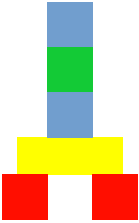
\includegraphics[scale=0.20]{figures/chapter2/task_goal.pdf}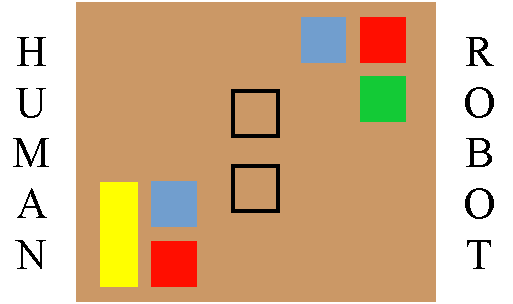
\includegraphics[scale=0.18]{figures/chapter2/task_setup_mini.pdf}}   
	\fancyhead[RO]{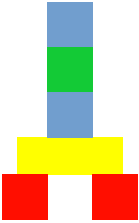
\includegraphics[scale=0.20]{figures/chapter2/task_goal.pdf}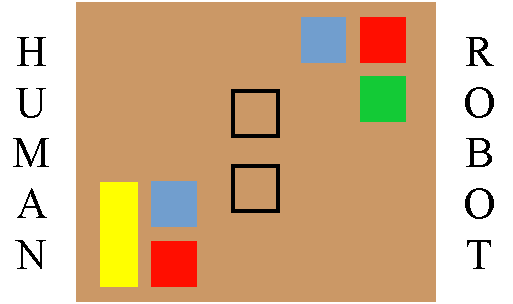
\includegraphics[scale=0.18]{figures/chapter2/task_setup_mini.pdf}\bfseries\thepage}  
	\fancyhead[RE]{\bfseries\nouppercase{\leftmark}}      % Chapter in the right on even pages
	\fancyhead[LO]{\bfseries\nouppercase{\rightmark}}     % Section in the left on odd pages
}%

\usepackage{pdfpages}
\usepackage{makecell}
\usepackage{pdflscape} 
\usepackage{mathtools}
\usepackage[section]{placeins}
\usepackage{afterpage}

%%%%%%%% my commands
\newcommand{\etal}{\textit{et al}.}
\newcommand{\ie}{\textit{i.e.}, }
\newcommand{\eg}{\textit{e.g.}, }
\newcommand{\fact}[3]{\mbox{\textit{#1}(#2, #3)}}
\newcommand{\circledtext}[1]{\raisebox{.5pt}{\textcircled{\raisebox{-.9pt} {#1}}}}
\newcommand{\sparql}{\textsc{SPARQL}}

\newcommand{\algConst}[1]{${\scriptscriptstyle #1}$}
\newcommand{\algNormTextSub}[2]{$\text{#1}_{#2}$}

\newcommand{\aslnumber}[1]{$#1$}
\newcommand{\aslstring}[1]{\textsf{#1}}
\newcommand{\aslvar}[1]{\textcolor{purple}{\textit{#1}}}
\newcommand{\asllabel}[1]{\textbf{#1}}
\newcommand{\annotation}[1]{{\footnotesize #1}}
\newcommand{\rulebody}[1]{\mbox{\hspace{.05\linewidth}}\begin{minipage}[t]{0.9\linewidth}#1.\end{minipage}}
\newcommand{\context}[1]{\begin{minipage}[t]{0.9\linewidth}#1\end{minipage}}
\newcommand{\planbody}[1]{\begin{minipage}[t]{0.9\linewidth}#1.\end{minipage}}
\newcommand{\Jason}[0]{\textbf{\textit{Jason}}}
\newcommand{\sn}{\mbox{\large\textbf{\texttt{\textasciitilde}}}}


\sloppy
\begin{document}
\setcounter{chapter}{1} %% Numéro du chapitre précédent ;)
\dominitoc
\faketableofcontents
\fi

\chapter{Joint Action-based Human-Aware supeRVISor: JAHRVIS}
\label{chapter:chap2}
\chaptermark{JAHRVIS}
\minitoc

In the previous chapter, we presented all the previous works we got our inspiration from, from psychology to robotics by way of philosophy, sociology and neuroscience. What is a social interaction? how can it be divided in steps? what is a joint action? how humans collaborate together? how do they take into account their partners? what happens when an agent makes a mistake? what has been done in computer science or robotics until now to make robots better collaborators? All these theories, ideas, questionings nourished our thoughts for the design and implementation of a supervision system dedicated to Human-Robot Joint Action. Supervision is key in the architecture as it is the robot decision kernel. And, as most components of a robotic architecture dedicated to \acrshort{hri}, one of the main issues of supervision is how to take the human into account, a more or less unpredictable agent with whom the robot has to collaborate. 

We presented in Section~\ref{chap1:subsec:state_art_sup} a few works tackling supervision issues, \ie how to adapt to the human, how to monitor them, how to face unexpected human behavior, how to optimize the task efficiency, how to make the robot an good human helper... They were very inspiring but we thought it was missing a general architecture and a software that could be used in different types of collaborative tasks, available for the community and that could easily be enhanced with new features. These thoughts led to the development of the \acrfull{jahrvis} which is the central topic of this chapter. We also came up with a novel idea: to endow the robot with the ability to measure if an interaction is going well or not. Such ability can be used by the supervision to enhance its adaptation capacity.

In the first section, we present the role and features we defined for \acrshort{jahrvis}. Then, in the three next sections, independent of each other, we lay the foundations for \acrshort{jahrvis} description. Indeed, in Section~\ref{chap2:sec:rob_archi}, we describe the robotic architecture in which \acrshort{jahrvis} is integrated. Next, in Section~\ref{chap2:sec:levels}, we present our representation of Human-Robot collaborative activity. And, as we made the choice to base \acrshort{jahrvis} on an existing BDI framework, we describe this latter in Section~\ref{chap2:sec:bdi}. Finally, we introduce \acrshort{jahrvis} architecture in Section~\ref{chap2:sec:jahrvis} whose role is to decide and control the robot during an interaction.

\section{The Role and Features of JAHRVIS}\label{chap2:sec:sup_features}

\acrshort{jahrvis} is a supervision system, \ie it embeds the robot high-level decisions, controls its behavior and tries to react to contingencies, whenever necessary considering the human it is interacting with. It is to differentiate from supervision systems dedicated to (multi-)robot control. It is able to do so by querying, managing and executing (shared) plans which are (partially) ordered set of actions to be performed by human and robot agents in order to achieve a (shared) goal. The plan management, described in Section~\ref{chap2:subsec:plan_handling}, is based on the estimation of the human's mental states, its knowledge about the current state of the environment, and recognized human actions. We explored the management of various kind of plans: 
\begin{inlineEnumerate}
	\item shared plans in which each action is allocated to an agent as well as action parameters are given objects,
	\item shared plans in which actions might not be allocated to an agent at planning time and parameters might refer to objects with a semantic query, and
	\item conditional plans which anticipate different possibilities for the human decision/action. 
\end{inlineEnumerate} 

As mentioned previously, the plan management relies on the recognition of human actions, among other things. \acrshort{jahrvis} integrates its own processes of action monitoring, \ie selecting the robot's point of interest and enabling joint attention, presented in Sections~\ref{chap2:subsubsec:robot_plan} and \ref{chap2:para:resource_m}, and of action recognition. This latter process, introduced in Section~\ref{chap2:subsec:h_moni}, is model-based and have been designed to be robust to a potentially unreliable perception of the human.

As there are actions of the plan to execute by the robot, \acrshort{jahrvis} needs interfaces with the robot controllers. Moreover, actions can be of two types, physical and communicative actions, and so requires a differentiated management. The methods implemented to handle the action execution will be introduced in Section~\ref{chap2:subsec:aem}.

Finally, an important feature is the ability to verbally communicate with the human. Indeed, during a collaborative task, communicate might be needed, among other things, to inform the partner of a performed action, or to ask them to perform one. Section~\ref{chap2:subsec:comm} describes the choices we made to endow the robot with a minimum set of communication abilities.

%Not only \acrshort{jahrvis} controls the robot contribution to a collaborative task, it also tries to evaluate if the interaction is going well or not. It is possible thanks to a set of metrics we have built and a method to aggregate them. We claim that having a robot with this ability allows it to enhance and make its decision-making processes more pertinent. The evaluation of the \acrlong{qoi} relies on a model of interaction, considered at  three levels: the interaction session level, the tasks level and the actions level. In future work, this granularity will allow the robot to know precisely on what level it needs to act when a low \acrshort{qoi} is assessed. Indeed, for instance, a task can be of poor quality while the session can still be considered as going well. \acrshort{qoi} principles and metrics will be described in Section~\ref{chap2:sec:qoi}.

\section{Design Methodology}

A part of the control features presented here is inspired from Sandra Devin~\cite{devin_2017_decisional}. Indeed, we intended to pursue her work, re-implementing a part of her software using Jason, a BDI framework presented in Section~\ref{chap2:sec:bdi}, instead of if/else statements in C++, giving our software more flexibility, readability and genericity.
Then, to go further, we developed \acrshort{jahrvis}, a more complete approach of a supervision component dedicated to HRI which tries to satisfy multiple requirements:

\begin{bulletList}
	\item \textbf{Be generic}. The objectives developed in the rest of list are to reach for most collaborative tasks. Thus, it seemed essential for us to develop a software not dedicated to a particular human-robot task but able to handle plans for varied tasks. 
	\item \textbf{Take into account the human partner}. In HRI, the human and the robot are partners. As seen in Section~\ref{chap1:sec:ja}, partners perform better when taking each other into account. Thus, by considering human abilities, perspective and mental states, the supervisor makes the robot a better partner for the human.
	\item \textbf{Leave decisions to the human}. In some cases, it is not useful, even counterproductive that the robot plans everything beforehand. Indeed, such elements such as the human action parameters, or who should execute a given action when it does not matter, or the order in which some actions should be executed, can be decided at execution time. Thus, we propose a supervisor handling two types of plan allowing to give latitude to human decisions and actions: conditional plans, and plans extending ``Agent X'' shared plans~\cite{devin_2017_decisions}.
	\item \textbf{Monitor human actions}. To monitor the plan progress, the robot should be able to monitor the human, \ie recognize their actions or be able to tell if they are idle.
	\item \textbf{Handle contingencies}. The robot has a shared plan, this is one thing, but to execute it and lead to the goal success is another one. Indeed, first, it is not sure that the human has exactly the same, and failures can happen (see Section~\ref{chap1:sec:failures}). Therefore, sometimes not everything is like the robot had planned and the decision and execution manager has to tackle this. Thus, it should be able to handle a certain amount of contingencies.
	\item \textbf{Manage relevant communications}. As stated in Section~\ref{chap1:subsec:comm}, communication is one of the key of collaboration. Therefore, it is important to endow the robot with the ability to manage relevant communication actions, verbal and non-verbal.
	\item \textbf{Consider the interaction outside collaborative tasks} A robot dedicated to collaborative tasks, in a real-life context, will interact with humans outside or between these tasks. We propose to consider this fact by defining what we called \textit{interaction sessions}. An interaction session gives a frame to the interaction and allows to take into account a number of facts from one task to another or from one session to another.
	\item \textbf{Adapt to the human experience, abilities or preferences}. Humans are all different, because of their experience, abilities or preferences among other things. A robot taking into account its previous interactions with a human (\eg behaving differently with a novel user or an experienced user) or adapting to their abilities (\eg some people cannot climb stairs, a robot guide can indicate the elevator instead) will improve the efficiency and the quality of the interaction, and the user's experience.
\end{bulletList}


\section{An Overview of the Robotic Architecture}\label{chap2:sec:rob_archi}

In this section, we will shortly present an overview of the robotic architecture that has been developed inside the RIS team of LAAS-CNRS. The purpose of this overview is inform the reader about the inputs available for \acrshort{jahrvis}. Two instantiations of this architecture for two different tasks will be described in Chapter~\ref{chapter:chap3} and Chapter~\ref{chapter:chap4}. This architecture model, shown in Figure~\ref{chap2:fig:archi}, has been inspired by the architecture developed by Lemaignan and colleagues~\cite{lemaignan_2017_artificial}, mentioned in Section~\ref{chap1:subsec:archi}. All communication between the components goes through ROS~\cite{quigley_2009_ros}.

\begin{figure}[!ht]
	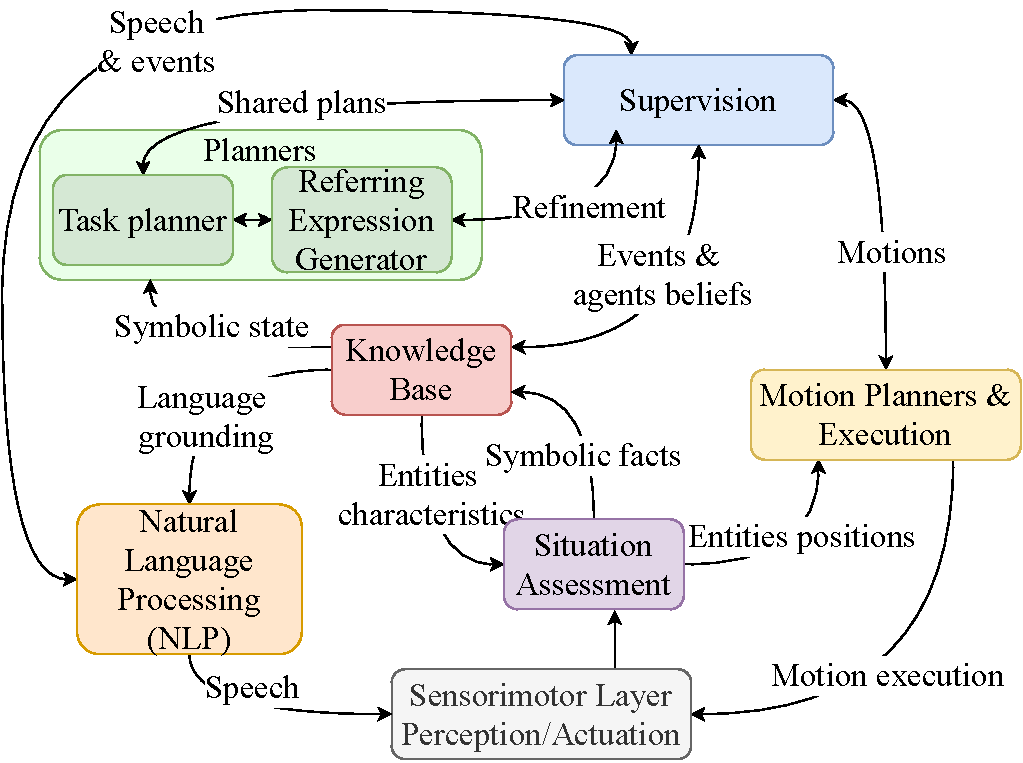
\includegraphics[width=\linewidth]{figures/chapter2/archi_overview.pdf}
	\caption{Overview of the RIS architecture}
	\label{chap2:fig:archi}
\end{figure}


\subsection{Situation Assessment}
The Situation Assessment has two roles:
\begin{enumerate}
	\item  to gather different perceptual information and build a geometric representation of the world (\ie elements have associated 3D coordinates), composed of objects and agents; from this world representation, the module runs reasoning processes to interpret it in terms of symbolic statements between the objects themselves and between the involved agents and the objects. Such component can be implemented with frameworks like Toaster~\cite{milliez_2014_framework} or Underworld~\cite{lemaignan_2018_underworlds}.
	\item estimate the human's perspective and build an estimation of their world representation; it is the first step allowing to implement the theory of mind principles (see Section~\ref{chap1:subsec:tom}).
\end{enumerate}

Thus, the Situation Assessment outputs data, which we call \textit{symbolic facts}, such as \fact{isOnTopOf}{cube\_1}{cube\_3} or \fact{isReachableBy}{cube\_2}{human\_0}. The first element of this triplet is called the property, the second one is the subject and the last one is the object.

\subsection{Knowledge Base}

During an interaction, each agent has their own knowledge base, as they can have belief divergences. A Knowledge Base is divided into two parts :
\begin{enumerate}
	\item The \textit{semantic} part is in charge of representing the environment elements meaning, the objects' and agents' types, their applicable properties, the descriptions and parameters of the actions, a part of the language model with verbs or pronouns, and their names in natural language. 
	
	Besides, it is also in charge of representing the current symbolic world-state (the computed facts) and thus the instantiation of the concepts in terms of physical (\eg this particular block) or abstract (\eg this particular action instance) entities.
	\item  The \textit{episodic} part is a timeline, keeping track of the symbolic facts computed over time, either by the Situation Assessment, the Semantic Knowledge Base or the Supervisor.
\end{enumerate}

The Supervisor can subscribe to a given type of fact, allowing to receive every fact update of this type. For example, the Supervisor can ask to receive every update (addition or deletion) of any fact belonging to the type \fact{isOnTopOf}{Cube}{Table}. In this case, it will receive the addition of \fact{isOnTopOf}{cube\_2}{table\_1} but not of \fact{isOnTopOf}{spoon}{table\_1}. It can also query an information when needed (\eg the Supervisor can ask the human understandable name of pick\_action which is ``pick'').

\subsection{Human-Aware Motion Planners and Execution}
The motion planners allow the robot to execute human-aware motion actions. According to the task needs, several planners might be involved for a same task. Indeed, in a task requiring object manipulation, the robot will need a motion planner able to plan for pick, place and drop actions, such as MoveIt\footnote{\url{https://moveit.ros.org/}} or GTP which is human-aware~\cite{waldhart_2016_novel}, and a home-made software handling the execution these trajectories\footnote{\url{https://github.com/YannickRiou/pr2_mtc}}. Moreover, in collaborative tasks, an agent might be led to hand over an object to their partner, in this case could be used a dedicated planner~\cite{mainprice_2012_sharing}. Finally, the robot might need to move in the environment, but when moving in a environment with humans, it should navigate being aware of them for safety and legibility. Thus, the robotic architecture should integrate co-navigation planner and executor such as HATEB-2~\cite{singamaneni_2020_hateb}. 

These planners produce trajectories and moves on request of the Supervisor. During execution, they sends feedbacks about the state execution, in this way the Supervisor can receive data about something going wrong or the estimated remaining time of execution. 

\subsection{Human-Aware Task Planner}
We can distinguish two situations in which a collaborative robot needs a human-aware task planner: 
\begin{inlineEnumerate}
	\item when it performs a task on its own but a human is nearby, and
	\item when it performs a task with a human.
\end{inlineEnumerate} 
In the first situation, it might consider asking the human's help whereas in the second one it needs to plan for both agents' actions. 

The human-aware task planner generates a shared symbolic plan in which each agent, human and robot, has actions of the task assigned to them, depending on some criteria. However, the human is neither an agent that the planner can directly control or an agent that will know the complete plan. Thus, it allows the robot to plan by emulating the human decision, action, and reaction processes. 

\subsection{Supervision}
The Supervision is the puppet master of the system, embedding the robot high-level decisions, controlling its behavior and trying to react to contingencies, always considering the human it is interacting with. It is not standalone, relying on the components described above to be able to take decisions, be aware of the environment and make the robot moves.
\newline

After giving an overview of the components on which the supervision relies, we present the context in which we place ourselves for human-robot collaboration.

\section{Representation of a Human-Robot collaborative activity}\label{chap2:sec:levels}
It is possible to describe and decompose a Human-Robot collaborative/joint activity in various ways for (see Section~\ref{chap1:subsec:def_ja} for discussions related to joint or collaborative activities). What we define as collaborative activities or tasks are types of joint actions. For all the following definitions, we place ourselves in the context of one-to-one human-robot interactions, however we  believe that the scheme can be extended to multi-human multi-robot contexts. 
We draw our inspiration from the literature of sociology and robotics, presented in Section~\ref{chap1:sec:soc_int} and Section~\ref{chap1:sec:soc_inter}, to define a model of interaction with three layered levels: interaction session, tasks and actions; as illustrated in Fig.~\ref{fig:levels}. We chose to represent collaborative tasks and their decomposition using the \acrfull{htn}~\cite{ghallab_2016_automated} representation which is often used in cognitive robotics~\cite{ingrand-2017,lallement_2014_hatp, buisan_2021_human} and because it allows to deal with goal-based and situation-based activities at different levels of hierarchy such as task, subtasks and actions and consequently to consider different levels of granularity. 

%In the example of a task with an overall bad Quality of Interaction, it would be interesting to know that in fact it is only a particular action or subtask ruining it. Indeed, the other parts of the task can be ok, or on the opposite, a particular subtask or action can have performed very well among the others. We need and use this granularity also on the three levels defined (interaction session, tasks and actions) to finely evaluate the Quality of Interaction, as a task can be of poor quality but the session is globally going well, \eg if a given task was a complete failed for some reasons but the other tasks were performed correctly. 

\begin{figure}[!ht]
	\centering
	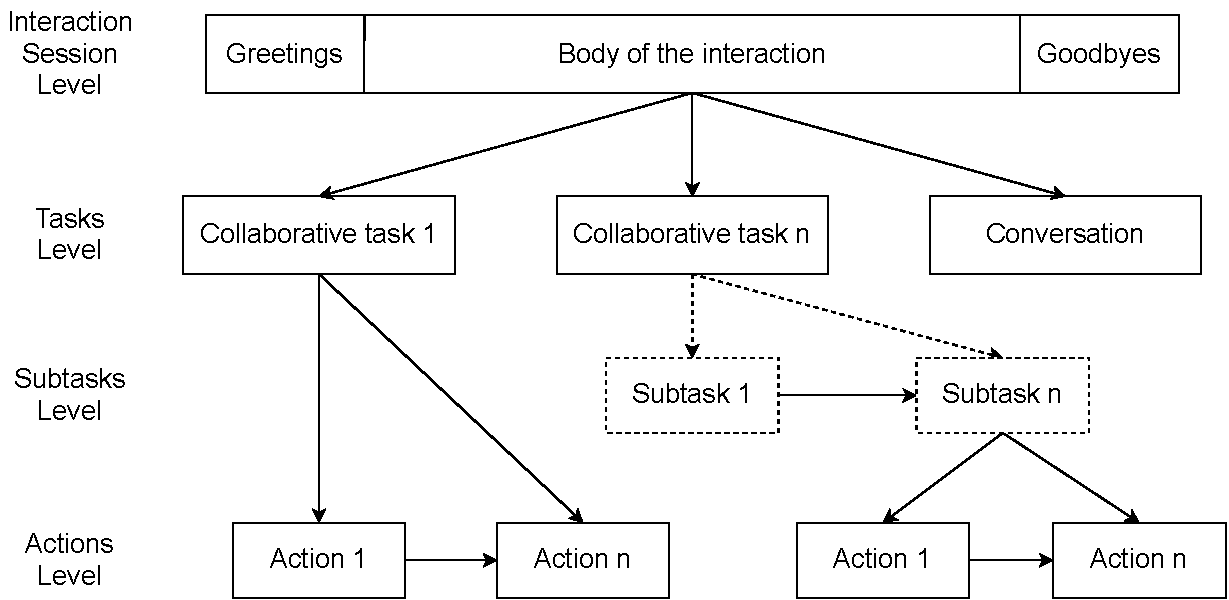
\includegraphics[width=\linewidth]{figures/chapter2/session_interaction.pdf}
	\caption{The hierarchical structure of an interaction session. The highest level is the interaction session. The second level is composed of the tasks. They are included in the body of interaction of the interaction session and, two types of tasks are considered and may overlap, collaborative and conversational tasks. With this representation, a task can be recursively refined as subtasks until reaching the last level, the actions level, which is considered as atomic.
%		Subtasks are not considered as a ``real'' level of the interaction session, specially to evaluate the \acrshort{qoi}, as it may exist or not according to the task.
		}
	\label{fig:levels}
\end{figure}


\subsection{Representation of a Human-Robot Interaction Session}
We define an \textbf{interaction session} as the period during which the robot and a human interact together and are engaged. It is divided in three parts, following the structure proposed by Robinson~\cite{robinson_overall_2012} as presented in Section~\ref{chap1:sec:soc_inter}: the greetings, the body of the interaction and the goodbyes. First, \textit{the greetings} corresponds to the period where an agent starts an interaction by initiating it with another agent. The interaction session lasts as long as the interactants are maintaining the interaction through conversation and collaborative tasks performance which corresponds to the \textit{body of interaction}. Finally it ends when at least one of the interactants is disengaged, either by abruptly ending the interaction or by closing the interaction as described by Schegloff and Sacks~\cite{schegloff_1973_opening}, it corresponds to ``the goodbyes''. For example, for an entertainment robot in a mall, an \textit{interaction session} starts when a person signals to the robot that they want to engaged, by greeting it or by approaching it and looking at it. The body of interaction is composed of conversation and eventually direction-giving tasks and, the session lasts until the person says goodbye or leaves. This is the nominal case and, the duty of the robot is to contribute to maintain the session alive until the human decides to close it, because it is at the service of humans. However, in some (extreme) cases, the robot might decide to close the interaction by itself.

Moreover, as seen in Section~\ref{chap1:subsubsec:joint_commit}, social interactions and joint activities (or actions) involve commitment, or rather engagement as we say in robotics -- this difference in the vocabulary as been highlighted in~\cite{castro_2019_commitments}. As explained in the previous chapter, there is no unique definition of what it means to be engaged. We chose one that is frequently used in robotics, proposed by Sidner and Lee~\cite{sidner_2003_engagement}: ``Engagement is the process by which two (or more) participants establish, maintain and end their perceived connection during interactions they jointly undertake''. The robot must be able to exhibit its engagement and disengagement and also to assess them with respect to its human partner.

We defined three states for the body of interaction, corresponding to what can happen during the latter: 
\begin{bulletList}
	\item conversation: a social chit-chat or a goal negotiation, without any physical action performed except communicative gestures
	\item collaborative task: both agents executing actions in order to achieve a shared goal
	\item idle phases: the agents are not chatting or performing a collaborative task together but remain engaged in the interaction session, it happens in-between active interaction phases
\end{bulletList}

For each of these three states, the way to exhibit the engagement varies (\eg in a conversation, an agent looking at their partner displays their engagement; during a task, an agent correctly performing their action is a way to demonstrate their engagement). That is why there is a need to define what behavior the robot has to exhibit in each state and what behavior it should expect from the human in each state, as these behaviors are usually very specific (\eg in a direction-giving task, the robot keeps its head oriented toward its partner's face to demonstrate its engagement in conversation and idle contexts and when it gives a direction it expects the human to look at the direction it is showing; in a stack task, when the robot gives an instruction it expects the human to take a given cube).

Transitions from one state to another can be managed by triggers more or less complex. For example, a collaborative task can be initiated when a human asks the robot that they achieve a goal together.


\subsection{Collaborative Tasks, Substasks and Actions}
\textbf{\textit{Tasks}} compose the body of the interaction of an interaction session as shown in Fig.~\ref{fig:levels}. We distinguish conversation (\ie agents engage in dialogue to exchange ideas, or to ask questions) from collaborative tasks (\ie agents work as partners, collaborating to perform tasks and to achieve common goals). We will not develop more on conversation since it is not the main focus of this work.

In joint or collaborative activities (see Section~\ref{chap1:subsec:def_ja}), humans are committed to achieve a goal together, involving collaboration and shared plans as shown in Section~\ref{chap1:sec:ja}. And, when interaction with a robot, the same mechanisms are also triggered as they are essential to a successful collaboration. When a human and a robot perform a task together, as described by Bauer \textit{et al}.~\cite{bauer_2008_collab}, we could say that the robot has the intent to help the human, so the human's intention becomes its own intention. Then, they have the joint intention to reach a common goal and, as shown by Michael and Salice~\cite{michael_2017_commitment}, they have a commitment to the joint activity, leading to perform joint actions. Therefore, during its evaluation and decision-making processes, the robot has to take into account that the human and itself should remain engaged all along an interaction session for the tasks to be successful and both have to manage and contribute to maintain expectations about what the other is doing. 

The elements composing a \textit{task} are: a goal, a plan and involved agents. A plan is needed to achieve a goal. There are many ways to generate a plan. But no matter the way (using a planner to anticipate execution or relying on a reactive planning scheme), we defined a plan as a sequence of actions in the end, even when it is hierarchical such as \acrshort{htn} plans. Sometimes, an abstraction higher than actions but lower than plan. So, we also define \emph{subtasks} or \emph{abstract tasks} which are sequences of actions, high level actions. 

\textbf{\textit{Actions}} are the elementary items of tasks, primitive tasks, manipulated by the high-level robot supervision controller. They cannot be decomposed further by it (\eg placement and motion planning are achieved by a lower control system not described here). It is usual to describe an action with its preconditions, its effects and, the agents and entities implied in its execution (\eg in plans written in PDDL (Planning Domain Definition Language)~\cite{ghallab_98_pddl}). We add to this description the notion of expected reactions (which can themselves be actions) from the other agents once the action is executed.

In our model, an agent (human or robot) is a contributor to the task and has a mental state as described by Devin \textit{et al}.~\cite{devin_2016_implemented}. The mental state is a set of facts representing, from the agent point of view, the current world state, the state of the goal and the current task state. Since we are interested here in the robot situation assessment and decisional processes, the mental state of the human is built and managed by the robot as an estimation of the beliefs of the human~\cite{milliez_2014_framework, hiatt_2017_modeling,tabrez_2020}.

\section{A BDI Framework as a Base of JAHRVIS Architecture}\label{chap2:sec:bdi}


\subsection{The Choice of the Programming Framework}
Restart from scratch or base oneself work on an existing software? This is the question which has been studied at the beginning of this thesis work about the implementation of the supervision software. It was possible 
\begin{inlineEnumerate}
	\item to develop the wanted features using the code\footnote{\url{https://github.com/laas/supervisor}} of the previous PhD student working on the supervision, Sandra Devin,\label{chap2:list:sandra}
	\item to choose among existing software dedicated to decision and execution for Human-Robot Interaction,\label{chap2:list:soft_hri}
	\item to choose among existing software dedicated to decision and execution for robotic platforms, and\label{chap2:list:robot}
	\item to develop a new software from scratch.\label{chap2:list:new}
\end{inlineEnumerate}

The obvious drawback of \ref{chap2:list:new} is that it takes a lot of time to start a new software from scratch and that it often leads to reinvent the wheel. Then, first we looked at existing solutions. Concerning the possibility \ref{chap2:list:sandra}, Devin had developed interesting features but the code is not modular and it was difficult to add new features or to modify the existing ones without breaking everything. Thus, there was the solutions \ref{chap2:list:soft_hri} and \ref{chap2:list:robot} left. When looking for existing software to manage human-robot interactions, we could not find any open-source one with a minimum of features, documentation and not entirely dedicated to a given task. Therefore, we turned ourselves toward robotic frameworks. We compared existing open-source decision-making and execution software for robots. To cite a few, there is the PetriNetPlans library introduced by Ziparo \etal~\cite{ziparo_2011_petri} which is a framework for planning and execution. Beetz \etal{} developed CRAM, a software implementing reasoning mechanisms that can infer control decisions~\cite{beetz_2010_cram}. A framework to implement hierarchical state machines is available among ROS libraries, SMACH\footnote{\url{http://wiki.ros.org/smach}}, defined as ``task-level architecture for rapidly creating complex robot behavior''. Or, a C++ library to create behavior trees has been developed, called BehaviorTree.CPP~\footnote{\url{https://github.com/BehaviorTree/BehaviorTree.CPP/}}. Finally, there are several implementations of the BDI model presented in Section~\ref{chap1:sec:archi} such as JAM~\cite{huber_1999_jam}, Jadex~\cite{braudach_2005_jadex}, SPARK~\cite{morley_2004_spark}, dMARS~\cite{dinverno_1998_formal}, OpenPRS~\cite{ingrand_1996_prs} or Jason~\cite{bordini_2007_jason}. 

As a first step, for prototyping and respecting project deadlines, our choice went to SMACH because its compatibility with ROS and its facility to be used. Then, it was no surprise, it became more and more difficult to program complex robot behaviors, state machine were not enough powerful. Thus, we examined possibilities for our second choice. After a comparison considering potential compatibility with ROS, possible integration with the other software of our architecture, availability of documentation, users' feedbacks, maintenance, and possibility of code modifications, our choice went to Jason designed by Bordini \etal~\cite{bordini_2007_jason} which is a Java interpreter of AgentSpeak created by Rao~\cite{rao_1996_agentspeak}. It has the advantage to be a BDI (Beliefs, Desires, Intentions, see Section~\ref{chap1:subsec:archi}) agent-oriented framework, fitting with our architecture. BDI frameworks implement a process, called the reasoning cycle or more commonly the sense-decide-act cycle~\cite{albus_1991_outline}, deciding step by step, which action to perform to reach a goal. It allows more modularity than state machines to handle contingencies and events. It also facilitates reasoning on agents' -- humans and robot -- beliefs. We chose this framework among the BDI ones and not another because it is implemented in Java and thus was compatible with rosjava\footnote{\url{https://github.com/rosjava/rosjava_core}} (\ie ROS implementation in Java), it is still developed and maintained, it is well documented (theoretically~\cite{bordini_2007_jason} and implement-ally\footnote{\url{http://jason.sourceforge.net/api/}}) which allows source code understanding and modifications, and there is a mailing list for users and its archives available\footnote{\url{https://sourceforge.net/p/jason/mailman/jason-users/}}.

\subsection{Programming with Jason}\label{chap2:subsec:jason}
As said above, Jason is a BDI-based framework, allowing what is called \textit{agent-oriented programming}. Originally designed for multi-robot programming, it can be used for other purposes such as ours. How does it work?

We explained in Section~\ref{chap1:subsec:archi} that there were three main concepts involved in BDI models: beliefs, desires and intentions. Well, Jason's purpose is to program agents. Thus, each agent has beliefs, desires and intentions. The beliefs are what it perceives, acquires from other agents and computes. They can produce desires, \ie states of affairs the agent wants to achieve. Then, the agent deliberates on its desires and choose to commit to some of them, \ie the chosen desires become intentions. To satisfy its intentions, the agent executes procedural programs, called plans, leading to actions. The procedural knowledge is written by the programmer.

The programming of the behavior of an agent is in the AgentSpeakLanguage (ASL). The program is designed by a user, a programmer. A program contains, among other things, plans. These plans have actions. An action is described by a Java program, written by the Jason's user. Then, to run, a program uses the decision loop, so called the \textit{reasoning cycle}, integrated to Jason. It is possible to customize some functions of the reasoning cycle by overloading or adding Java functions of the agent's constructors, belief base and reasoning cycle. 

\subsubsection{Agents} In the ASL program of an agent, it is possible to see plans, beliefs, desire and test goal. First, let's see a very simple example of program with the agent Bob\footnote{\url{http://jason.sourceforge.net/mini-tutorial/hello-bdi/}}, presented in Listing~\ref{chap2:lst:bob}. Bob has one initial (\ie given by the programmer, not acquired by perception) belief which is |happy(bob)|. A belief is a property, here |happy|, which can have whatever number of arguments (including zero), here |bob| and a source (\eg |source(percept)| means that the belief has been acquired through perception, |source(self)| means that it has been computed by the agent itself and |source(alice)| means that it has been received from the agent Alice). Then, he has one initial desire which is recognizable by |!|. And finally, he has a plan allowing to achieve the desire |say(hello)|. A plan is triggered by an event, here |+!say(X)| (\ie the event is that the goal |say(hello)| has been added), has a context (\ie a precondition), here |happy(bob)| and has a body which contains the actions to execute, here |.print(X)| (with |X| being a variable -- variables have their first letter in upper case). If we remove the initial belief |happy(bob)| from the first line, as the program is written and considering that Bob is the only agent, he cannot print hello, as the precondition of the plan will not be true.

\begin{lstlisting}[caption={ASL program of Bob, a Jason agent}, label={chap2:lst:bob}]
happy(bob).	\\belief

!say(hello).	\\desire

\\plan
+!say(X) : happy(bob) <- 
	.print(X).		
\end{lstlisting} 

In another example, illustrated by Listing~\ref{chap2:lst:bobalice}, Bob has no initial belief nor initial goal. He has plans for two events: starting to believe he is happy and having the goal to say hello. We can see that there is also a program for another agent, Alice. She has an initial goal, her, which is to inform bob that he is happy. Therefore, we can see that an agent can add a belief in another agent's belief base. When Bob gets the information that he is happy, this triggers his first plan, creating for him the goal |!say(hello)|. As Bob does not believe that today is Monday, he can trigger his second plan to say hello. In this plan, there a three elements: a print action, a wait action and the addition of a new goal. And thus, here, we are in the presence of a recursive plan which never ends. 

\begin{lstlisting}[caption={ASL programs of Bob and Alice, two Jason agent}, label={chap2:lst:bobalice}]
\\bob.asl
\\for example purposes, the precondition is true
\\but it can be logical expressions with beliefs,
\\functions...
+happy(bob) : true <- 
	!say(hello).

+!say(X) : not today(monday) <- 
	.print(X); 
	.wait(500); 
	!say(X).

\\alice.asl
!inform.

+!inform : true <- .send(bob,tell,happy(bob)).
\end{lstlisting} 

\subsubsection{Actions} To give an idea of what looks like the Java program of an action, here is an example of a Java function for the action |.print| in Listing~\ref{chap2:lst:print}.

\begin{lstlisting}[caption={.print action}, label={chap2:lst:print}, language=Java]
public class print extends DefaultInternalAction {
	@Override
	public Object execute(TransitionSystem ts, Unifier un, Term[] args) throws Exception {
		String sout = argsToString(args);
		System.out.print(sout.toString() + "\n");
	}
	return true;
	}
}
\end{lstlisting} 

In Jason, there are two types of actions defined: \emph{environment actions} and \emph{internal actions}. \emph{Environment actions} allow an agent to act within its environment, usually producing effects visible by other agents. Whereas, \emph{internal actions} are designed to be run internally within an agent such as the print action and can be used to return values or booleans. When being executed, there are not handled the same way in the Jason's reasoning cycle. The definition of which type an action should be falls to the programmer, which should choose according to their need.

We have seen what looks like the program of Jason agent. Now, we are going to see how it is run by the Jason interpreter.


\subsubsection{Reasoning cycle} Each agent has what has been coined a \textit{reasoning cycle}, composed of 10 steps. It resembles a decision loop, running each step one by one and starting again at the first one. The steps 1 to 4 are dedicated to the belief update of the agent. The steps 5 to 10 describe the interpretation of the ASL program. In these latter, an event is selected, as well as a plan corresponding to this event and then the first formula (\eg an action or a goal) of the plan is executed. It is illustrated by Figure~\ref{jason_cycle}. The steps are the following ones, in this order:
\begin{enumerate}
	\item Perceiving the Environment: Each agent has a Java function called |perceive|. This function can retrieve data from a simulated environment or be customized by the programmer to get actual perception data. The function outputs a list of beliefs, along with their source (\eg |<isOn(box1,table)[source(percept)]|, |color(box1,red)[source(percept)]>|).
	\item Updating the Belief Base: The agent's belief base is updated with the perception data. Each change in the belief base generates an event (\eg |+color(box1,red)[source(percept)]| and if later the color of the box is not part of the perception data anymore, it will be |-color(box1,red)[source(percept)]|).\label{chap2:list:update_bb}
	\item Receiving Communication from Other Agents: It checks if an agent received a message from another agent such as the message Bob received from Alice in Listing~\ref{chap2:lst:bobalice}. A message can be a belief, a plan, a goal or a questioning on a given belief.
	\item Selecting ‘Socially Acceptable’ Messages: It is a function the programmer should customize. It allows agent to refuse messages or types of message from some given agents based on some rules written in Java by the programmer, \eg no message from the agent Alice.
	\item Selecting an Event: Events are either perceived changes in the environment or changes in the agent's own goals. There is a queue of events and at each reasoning cycle only one is selected to be handled. The default method to select it is a FIFO but, as every function of the reasoning cycle, it can be customized. 
	\item Retrieving all Relevant Plans: From the selected event, it tries to find all the relevant plans for this event, in the plan library, \ie the plans written by the programmer in ASL. The function tries to find the plans that can be \textit{unified} with event, \ie the ones with their left part (the trigger) matching the event. For example, if the selected event is |+color(box1,red)[source(percept)]| and in the plan library there are these six plans:
\begin{lstlisting}[style=inline]
+position(Object,Coords) : true <- .print(Coords).
+color(Object,red) : true <- .print(nice).
+color(Object,red)[source(self)] : true <- .print(nice).
+color(box1,Color) : true <- .print(nice).
+color(Object,Color) : false <- .print(Color).
+color(Object,blue) : true <- .print(so-so).
\end{lstlisting}
	then there are three relevant plans (the last one is also relevant because what is looked for here is the triggers only and not the preconditions):
\begin{lstlisting}[style=inline]
+color(Object,red) : true <- .print(nice).
+color(box1,Color) : true <- .print(nice).
+color(Object,Colour) : false <- .print(Colour).
\end{lstlisting}
	\item Determining the Applicable Plans: It takes the list of relevant plans and sees which ones are applicable. To do so, it looks at the context (the preconditions) of the plans. The context can be beliefs, prolog-like rules, internal actions, logical expressions or booleans. If we look at the example of the previous step, there were three relevant plans. Their contexts are simple booleans. Two of them are true, the other one is false, thus the two first plans are applicable.
	\item Selecting One Applicable Plan: It takes the list of applicable plans and selects the one that will be elected to become an intention, \ie to be executed. As usual, this is a customizable function for which the default behavior is to take the first plan in the order of the plan library, \ie in the order written by the programmer. Still with the same example, thus, the one plan to be selected is the first one, |+color(Object,red) : true <- .print(nice).| If the event was external, \ie from perception, it creates a new intention, adding it to the set of intentions. Then, the agent has a new \textit{focus of attention}. If the event was internal, \eg a belief addition inside a plan, then the selected plan is added on the top of the existing intention. 
	\item Selecting an Intention for Further Execution: As seen in the previous step, an agent can have more than one intention in the set of intentions, each representing a different focus of attention. Then, at this step is chosen the intention of which the formula will be executed. The default function chooses the first intention of the list. After execution of the formula, the intention will go at the end of the intentions list.
	\item Executing One Step of an Intention: The first formula of the selected intention is executed (this number is also customizable and the programmer can choose that an agent execute more than once formula in the same reasoning cycle). It can be an internal action, an environment action, a goal, a belief addition or deletion and two other types that will not be developed here. 
\end{enumerate}

Therefore, each agent has a reasoning cycle running repeatedly, independent from the other agents' reasoning cycle. Interactions between each agents happen through the messages they send to each others and eventually the effects they produce on the environment which are then perceived by the other agents. 


\begin{landscape}
\begin{figure}
	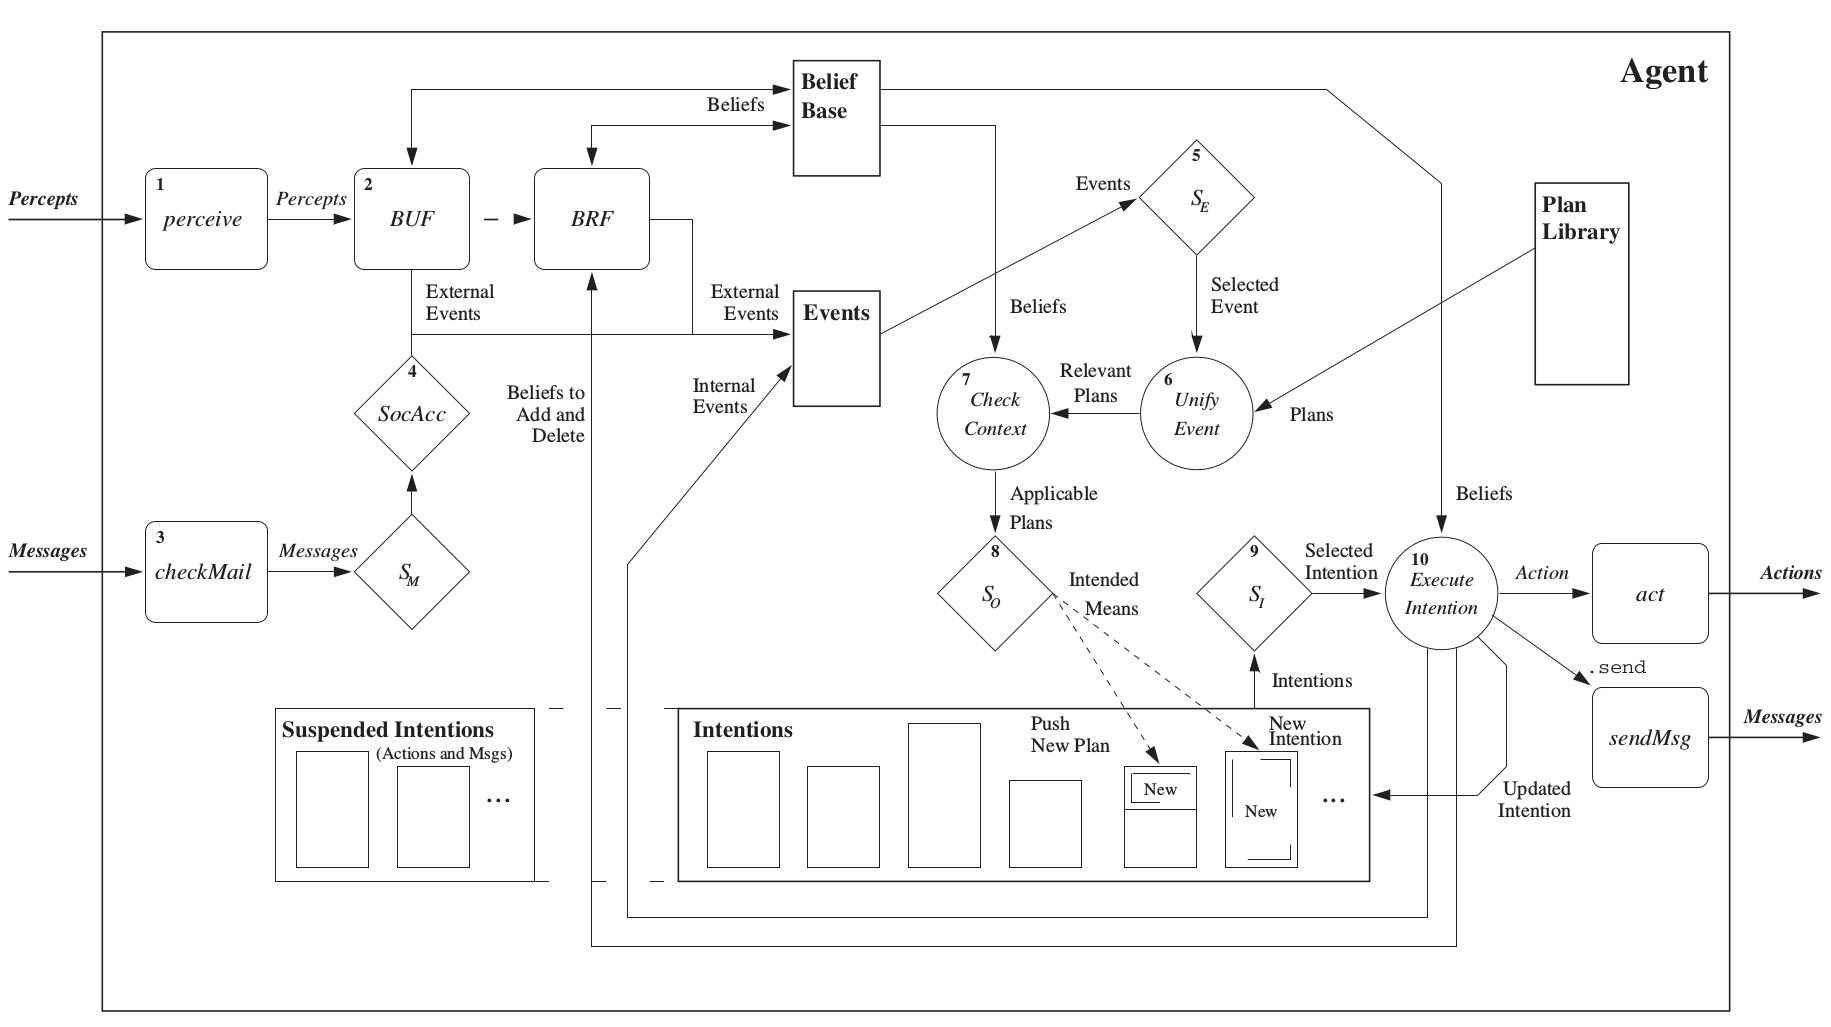
\includegraphics[width=\linewidth]{figures/chapter2/jason_cycle.png}
	\caption{The Jason reasoning cycle~\cite{bordini_2007_jason}. Each step presented above has its numbered corresponding box.}
	\label{chap2:fig:jason_cycle}
\end{figure}
\end{landscape}

\subsubsection{Plan failure handling}

For the case where a plan fails (\eg an action fails -- there are other reasons for which a plan could fail but we will not discuss the details here), Jason integrates a mechanism handling failures. It consists in cancel the execution of the plan and generating a triggering event for a contingency plan whose prefix is |-!|. If the contingency plan can be found -- written by the programmer --, it is executed. Then, if the plan which originally failed was a subplan of another plan, this plan will continue normally. 

An illustration is given in Listing~\ref{chap2:lst:failure}. The result of the execution of this agent file would be the printing ``unknown error'' and then ``bye'' in case of the failure of the |robot_speech| action execution with an instantiated speech module. Indeed, the initial goal |speak| creates the subgoal |say_hello|. Unfortunately, the action |robot_speech| fails with an empty error message, generating the event |-!say_hello[error_msg(Msg)]|. There are two plans for this event but as |Msg=""|, the second one is chosen, printing ``unknown error''. Then, |speak| continues in the same way it does when goal |say_hello| is achieved successfully, printing ``bye''.

\begin{lstlisting}[caption={Example of plan failure handling}, label={chap2:lst:failure}]
!speak.

+!speak : true <- 
!say_hello;
.print(bye).

+!say_hello : true <-
robot_speech(hello);
.print(hello).

-!say_hello[error_msg(Msg)] : .substring(Msg,no_speech_found) <-
.print(no speech module was found).

-!say_hello[error_msg(Msg)] : true <-
.print(unknown error).	
\end{lstlisting} 

\subsection{Jason Integration with ROS}
The robotic architecture presented in Section~\ref{chap2:sec:rob_archi} uses the ROS framework~\cite{quigley_2009_ros} to enable communication between its components. Thus, to be able to build a supervision software based on Jason, we needed to interface it with ROS as well. At the time, there was no available bridge between Jason and ROS, Jason being extensively used in simulation contexts. Thus, we developed our own -- and at about the same moment, the Jason's developers started to develop theirs~\cite{silva_2020_embedded} (what we realized a bit later), both using rosjava. We tackled the problem in very different ways. A user of their implementation only needs to fill one perception (topics) and one action (topics/services) manifests to link the system with ROS and then implement their agent in ASL. Thus, it is quite easy to use. However, it has drawbacks. Therefore, action requests are directly sent from ASL to the hardware controller, with no possibility of Java processing. Moreover, action status/result can only be boolean which is not enough for a system like ours needing to perform service queries of data to the external Knowledge Base for example. Finally, there is no bridge with action servers which are often used for motion planers for example. 

\begin{figure}[!ht]
	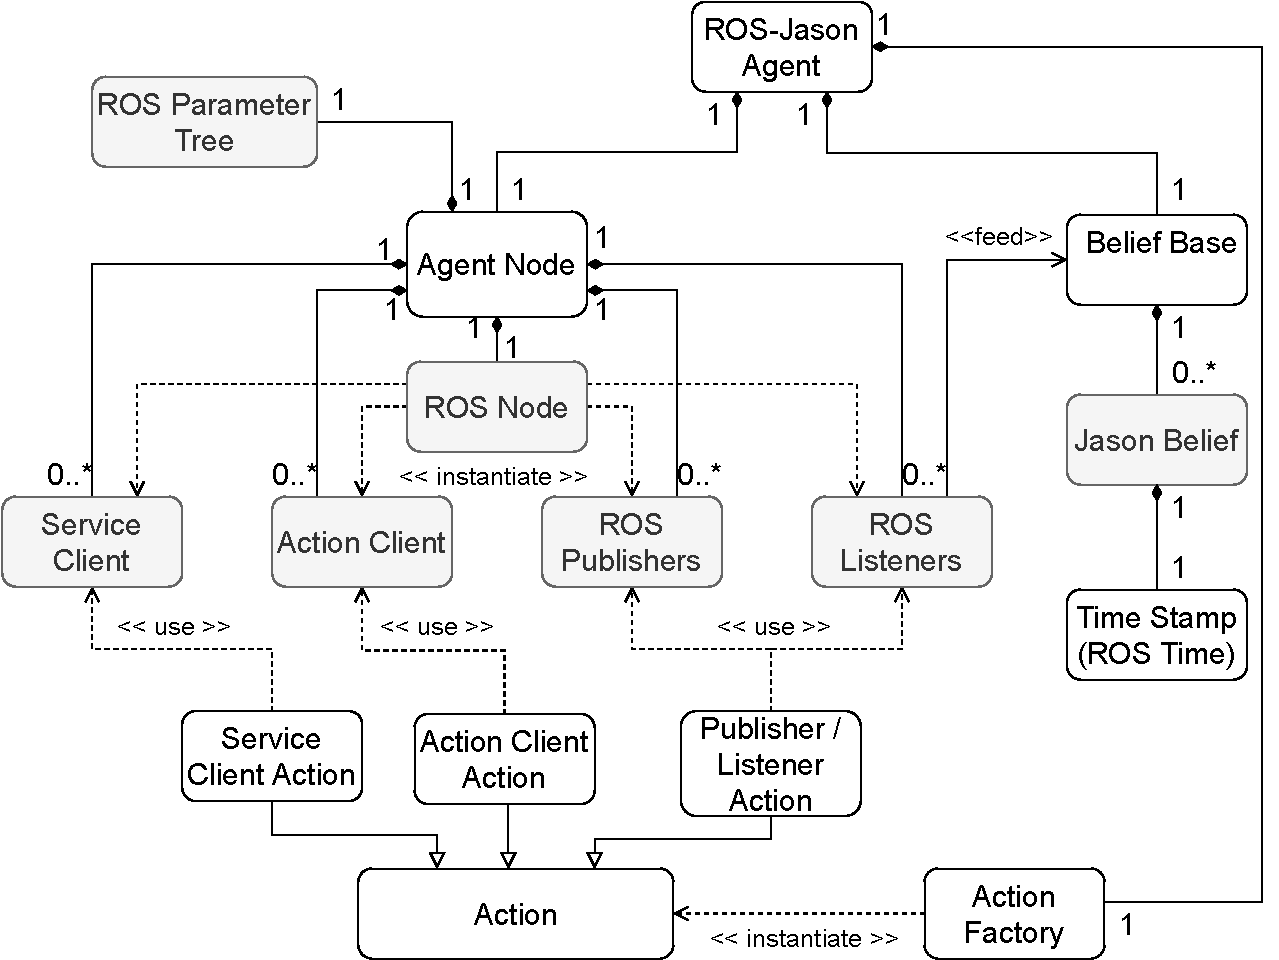
\includegraphics[width=\linewidth]{figures/chapter2/RJS_diagram.pdf}
	\caption{Simplified Java class diagram of our ROS-Jason implementation. In white are our customized classes and in grey the native ROS and Jason classes.}
	\label{chap2:fig:rjs}
\end{figure}

A simplified Java class diagram of our  implementation\footnote{\url{https://github.com/amdia/rjs}} is presented in Figure~\ref{chap2:fig:rjs}. We defined for each Jason agent a customized Java class (\acrfull{rja} on the figure) which has an Agent Node, an action factory and a belief base where all beliefs are time stamped with the roscore time. 

An Agent Node has an attribute, the ROS Parameter Tree, allowing to load YAML parameters from files in which, among other things, are written services, topics and action servers info, as shown in Listing~\ref{chap2:lst:ros-jason}, a bit similarly to the manifests of~\cite{silva_2020_embedded}. From these parameters, the Agent Node can automatically instantiate all the needed ROS components through its ROS node. 

The Belief Base can receive perception updates through ROS topic listeners. Moreover, we customized\footnote{This modification of the belief update function is not part of our ROS-Jason implementation but is on top of it, in the \acrshort{jahrvis} implementation which relies on ROS-Jason.} the belief update function (step~\ref{chap2:list:update_bb} of the reasoning cycle) as we chose to abandon a state-based perception to adopt an event-based perception. So, percepts are not elements that when perceived at time T are added to the belief base and disappearing when not perceived anymore at time T+1. There are now updates (additions and deletions) from the external Knowledge Base, in this way, it limits the number of message exchanges, \ie instead of receiving every 500 ms during 10 seconds that the agent perceives |cube_1|, it receives for example an addition at t=18s and a deletion at t=28s. 

To each belief added in the belief base, from perception or internal computation, is added a time stamp from the current ROS time. Currently, it is useful for the computation of the Quality of Interaction presented in Section~\ref{chap2:sec:qoi} and for debugging but it could have other uses such as \todo{??}

An \acrshort{rja} has an Action Factory -- abstract in the ROS-Jason framework and instantiated in \acrshort{jahrvis} -- containing the list of environment actions it can perform -- in the case of our architecture, not all actions of this type are for the robot to act on its environment, sometimes there are queries to other components of the architecture. The Action Factory instantiates the Action called through the ASL program at execution time. An Action can either be based on a ROS service client, or an ROS action client, or a ROS publisher for the request and a ROS listener for the result. 

\begin{lstlisting}[caption={Example of service, topic and action server definitions in a YAML file.}, label={chap2:lst:ros-jason}]
services:
	onto_individual: 
		name: /ontologenius/individual/robot
		type: ontologenius/OntologeniusService
	onto_class: 
		name: /ontologenius/class/robot
		type: ontologenius/OntologeniusService
topics:
	mementar_occasions: 
		name: /mementar/occasions/robot
		type: mementar/MementarOccasion
		function: sub
	plan_request:
		name: /planner/request_new_plan
		type: planner_msgs/PlanRequest
		function: pub
action_servers:
	plan_motion: /pr2_tasks_node/plan
	execute_motion: /pr2_tasks_node/execute
\end{lstlisting}


\section{The Architecture of JAHRVIS}\label{chap2:sec:jahrvis}
The \acrfull{jahrvis} is implemented on top of our ROS-Jason framework\footnote{\url{https://github.com/amdia/ld_rjs}}. During the design of \acrshort{jahrvis}, we identified seven high-level features we needed and implemented their associated processes, based on the objectives presented in Section~\ref{chap2:sec:sup_features}\footnote{The design of \acrshort{jahrvis} was an iterative work, indeed the first version being the supervisor implemented for the task described in Chapter~\ref{chapter:chap3}, the second one was the supervisor of the task described in Chapter~\ref{chapter:chap4} and the final one was the supervisor of the task described in Chapter~\ref{}}\todo{to update later}. We present \acrshort{jahrvis} architecture in Figure~\ref{chap2:fig:sup_overview}, with the seven processes in blue, the \acrshort{qoi} Evaluator dedicated to the interaction evaluation and the six others to the decision and control. All the next developments of this chapter will be about the description of these processes.

\begin{figure}[!ht]
	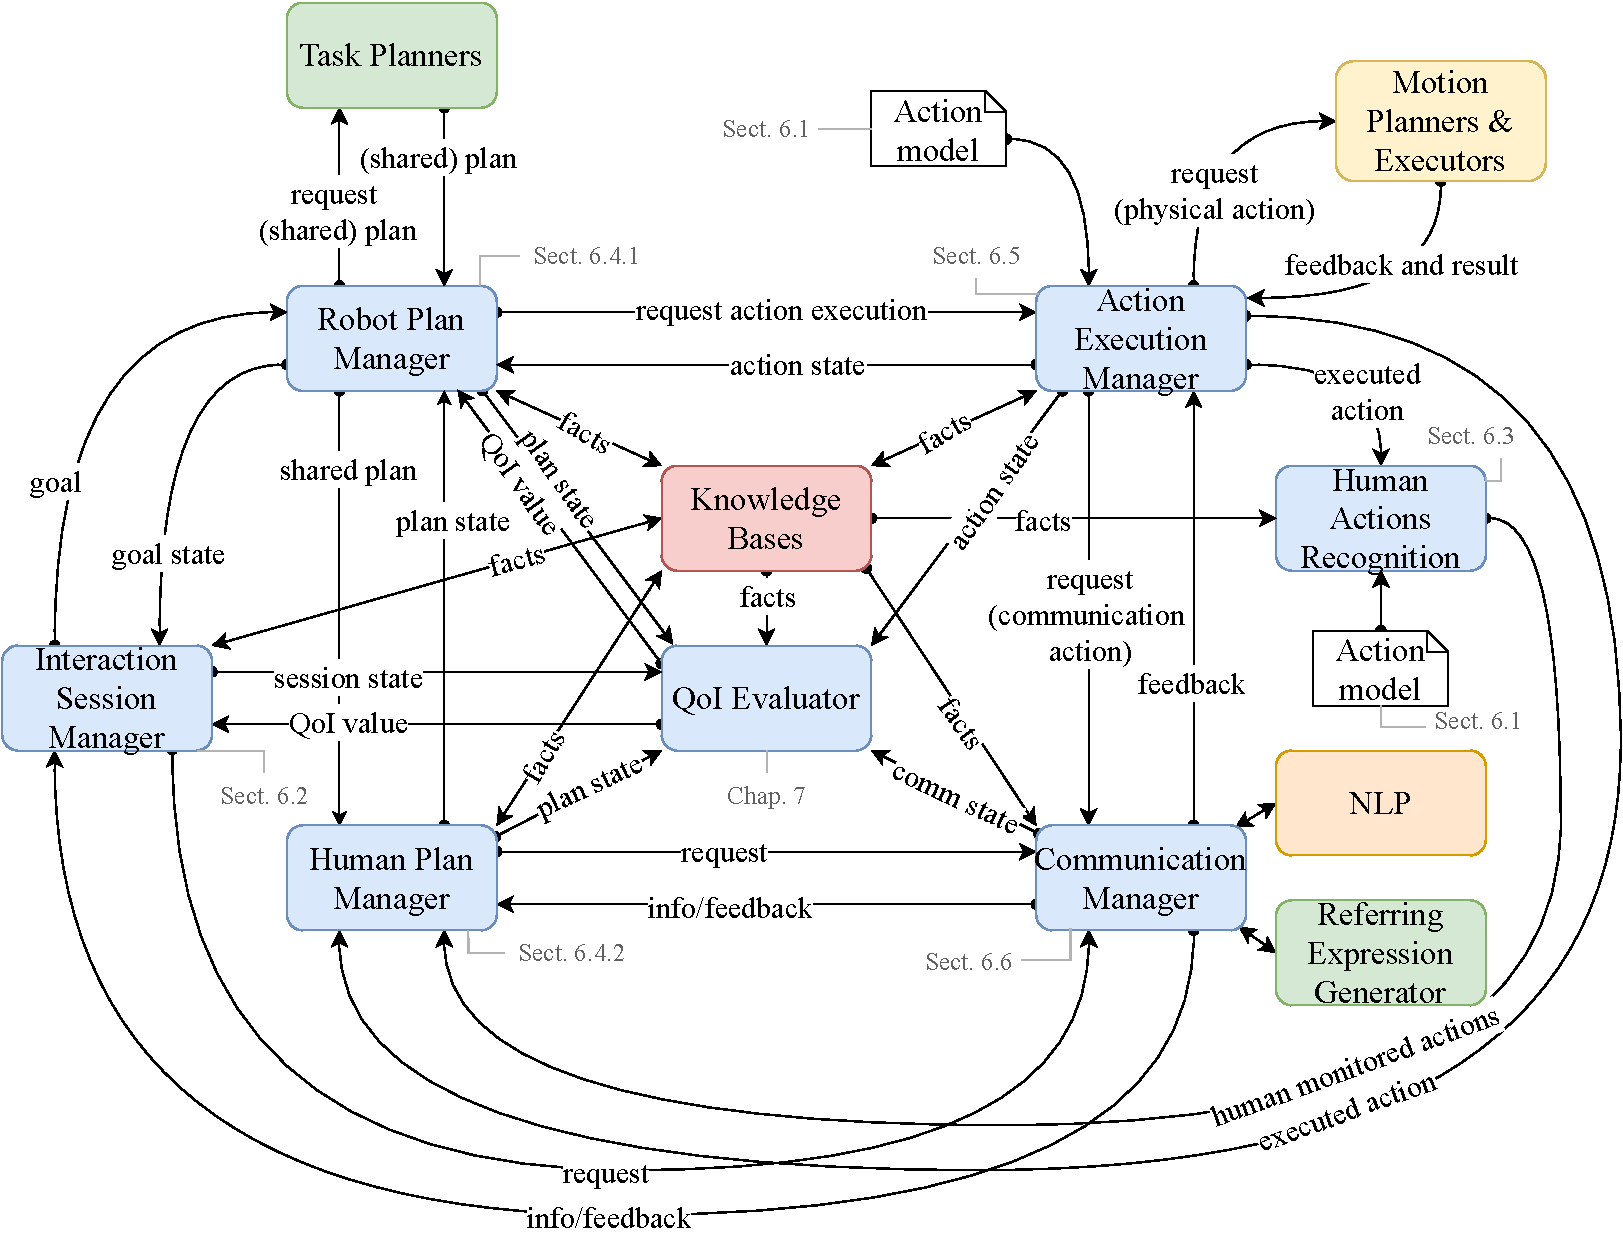
\includegraphics[width=\linewidth]{figures/chapter2/supervisor_modules.pdf}
	\caption{The \acrshort{jahrvis} processes (in blue) and their interactions between themselves and with the other components of the robotic architecture presented in Section~\ref{chap2:sec:rob_archi}.}
	\label{chap2:fig:sup_overview}
\end{figure}

For each process (in blue in Figure~\ref{chap2:fig:sup_overview}), we implemented an \acrshort{rja}, with the desired behavior coded in ASL and the needed customizations added in Java. Thus, internal communications between the \acrshort{jahrvis} processes, and so \acrshort{rja}s, use Jason messages (see Section~\ref{chap2:subsec:jason}). External communication with the other components of the robotic architecture is based on either ROS messages, services or action clients.

Not all \acrshort{rja}s are active at each level of interaction defined in Section~\ref{chap2:sec:levels}. Indeed, as its name suggests, the \textit{Interaction Session Manager} handles interaction sessions. The \textit{Robot} and \textit{Human Plan Managers} handle the task level. And, the \textit{Action Execution Manager} and the \textit{\acrlong{ham}} are in charge of the action level. The \textit{\acrshort{qoi} Evaluator} and the \textit{Communication Manager} are active at all levels. We can also make the distinction between the component dedicated to the assessment of the quality of interaction, \ie the \acrshort{qoi} Evaluator, and the components dedicated to the decision-making and control, \ie all the components except the \acrshort{qoi} Evaluator.

In the Sections~\ref{chap2:sec:control} and \ref{chap2:sec:qoi} will be presented these processes. Section~\ref{chap2:sec:control} introduces the ones related to the decision-making and robot control while Section~\ref{chap2:sec:qoi} describe the evaluation process of the \acrlong{qoi}. Section~\ref{chap2:sec:control} will start by laying the foundations for the \acrshort{rja} functioning: the knowledge representations and management. Then, each \acrshort{rja} will be thoroughly described. The \acrfull{ism} is dedicated to in-between tasks, \ie the opening and closing of interactions and all the dialog which can happen between two collaborative tasks. When a shared goal is established, the shared plan is handled by the \acrfull{rpm} and the \acrfull{hpm}, \ie to follow the plan progression, to make sure that the observed human actions match the ones of the plan and to decide when the robot should act. Robot actions to perform are sent to the \acrfull{aem} that interfaces with the motion planer and executor. As for human actions, they are monitored and recognized by the \acrfull{ham}. Finally, the \acrfull{cm} is in charge of producing the communication for the human when requested by another \acrshort{rja} along with the human communication reception.


\section{A robot controlling its contribution to a human-robot joint action}\label{chap2:sec:control}\todo{related work}

The objective of this section is to present the \acrshort{jahrvis} processes involved in the decision-making and the control of the robot when jointly interacting with a human. First, we present the knowledge representations used, then the \acrlong{ism}, the \acrlong{ham}, the Shared Plans Handling composed of two processes, one for the robot (\acrlong{rpm}) and one for the human (\acrlong{hpm}), the \acrlong{aem}, and finally the \acrlong{cm}.

\subsection{Knowledge Representations and Management}\label{chap2:subsec:know}
As shown in Section~\ref{chap1:subsubsec:shared_rep} and Section~\ref{chap1:subsubsec:common_g}, when involved in joint actions, humans have shared representations of tasks, actions, goals and have a common ground. Thus, it is important that the robot has such internal representations.

During an interaction, \acrshort{jahrvis} processes use knowledge bases (KB) of two types: external and internal ones. The external knowledge bases with which we interfaced \acrshort{jahrvis} are Ontologenius\footnote{\url{https://github.com/sarthou/ontologenius}}~\cite{sarthou_2019_ontologenius} for the semantic knowledge and Mementar\footnote{\url{https://github.com/sarthou/mementar}} for the episodic one. They have been developed by Guillaume Sarthou with whom we collaborated closely. A reason for this choice is that it is fully adapted to HRI applications by representing the robot's knowledge and the estimation of the partners' knowledge separately, which refers to the psychological concept of the ``self-other distinction'' as coined in joint action studies~\cite{pacherie_2012_agency}. 

Moreover, each \acrshort{rja} has its own knowledge base that we call belief base in Jason vocabulary. It is used for knowledge which serves to \acrshort{jahrvis} internal computations only.

Ontologenius allows to store common-sense knowledge (\eg a cube is an object), knowledge about the environment (\eg object\_1245 is a Cube and is on top of table\_2) and knowledge about activities grounded in space and time (\eg object\_1245 has been put on the table\_2 by robot (action ID 475)). Mementar allows to store facts and actions in a timeline (\eg action ID 475 started at 3286 seconds and was over at 3290 seconds). As stated in Section~\ref{chap2:sec:rob_archi}, it receives and stores facts about the current state from the Situation Assessment component. It reasons on it, making some deductions and links between facts, creating new ones (\eg after receiving \fact{isOnTof}{cube\_2}{table\_1} and it computes \fact{isUnder}{table\_1}{cube\_2}). 

The knowledge representation in Ontologenius is based on three concepts: (1) classes representing the possible types of entities known by the agent (\eg Cube is a class inheriting from the class Pickable), (2) properties which can denote both the attributes of objects (\eg the color) and the relations between the objects (\eg which object is on which other one), and (3) object instantiations also called individuals (\eg cube\_3 is an object present in the environment, of the class Cube).

To access to the knowledge stored in Ontologenius, \acrshort{jahrvis} can make a request to know if a given fact exists or ask an information about a class, a property or an object instantiation. Another way is to subscribe to updates (addition or deletion) for a given fact. It is useful for keeping updates about the environment and avoid to be snowed under too much data (\eg to monitor human place actions, \acrshort{jahrvis} needs \textit{isOnTopOf} but not \textit{isUnder} so \acrlong{ham} can subscribe to updates about this first fact). It is possible to either specify the class or individual of the subjects/objects that should be concerned by the subscription, or to receive every facts (\eg it can subscribe to receive additions of the human looking at the robot |[add]human_0$\lvert$isLookingAt$\lvert$robot| or to receive all updates about every objects that the human looks at |[?]human_0$\lvert$isLookingAt$\lvert$?|).

\subsubsection{Action Representations}\label{chap2:subsubsec:action_rep}
Action representations allow the robot to recognize actions, to execute actions, to monitor the human monitoring its actions and to communicate about them. We defined three action representations according to their use. We chose to have one stored in Ontologenius to benefit from the reasoning features and to have the two others written in an ASL file to benefit from Jason reasoning features.

\paragraph{External Action Representation}
For the needs of \acrshort{jahrvis}, we represented actions, their verbal labels and their effects in a semantic \acrshort{kb} in the form of an ontology\footnote{An ontology is a way to represent knowledge} managed by Ontologenius. We show in Figure~\ref{chap2:fig:class_actions} a representation of some actions we stored in Ontologenius using the Web Ontology Language (OWL) (see Listing~\ref{chap2:lst:classes}) and in Figure~\ref{chap2:fig:class_effects} a representation of possible action effects.

\begin{lstlisting}[style=OwlTurtle, label={chap2:lst:classes}, caption={Description of ontology classes in the OWL language using the Turle syntax.} ]
:PhysicalAction	rdf:type owl:Class ;
				rdfs:subClassOf :HtnAction .

:ScanAction	rdf:type owl:Class ;
			rdfs:subClassOf :PhysicalAction ;
			htn_actions:hasEffect :IsScannedEffect ;
			rdfs:label ``{Agent} @Scan {Pickable}'' .

\end{lstlisting}

One of the advantages of using action model stored in Ontologenius is the class inheritance. It allows to define properties for one class that will be transmitted to its child classes (\eg if it exists multiple class representing a drop action, let's say |human_drop_cube| and |robot_drop_cube|, both inherit from the properties of |DropAction| such as the label used for the action verbalization). Another advantage is to be able to link classes through properties and to easily query the \acrshort{kb} about it (\eg what are the effects of the |PickAction| and then what types of effects are they?).

\begin{figure}[!ht]
	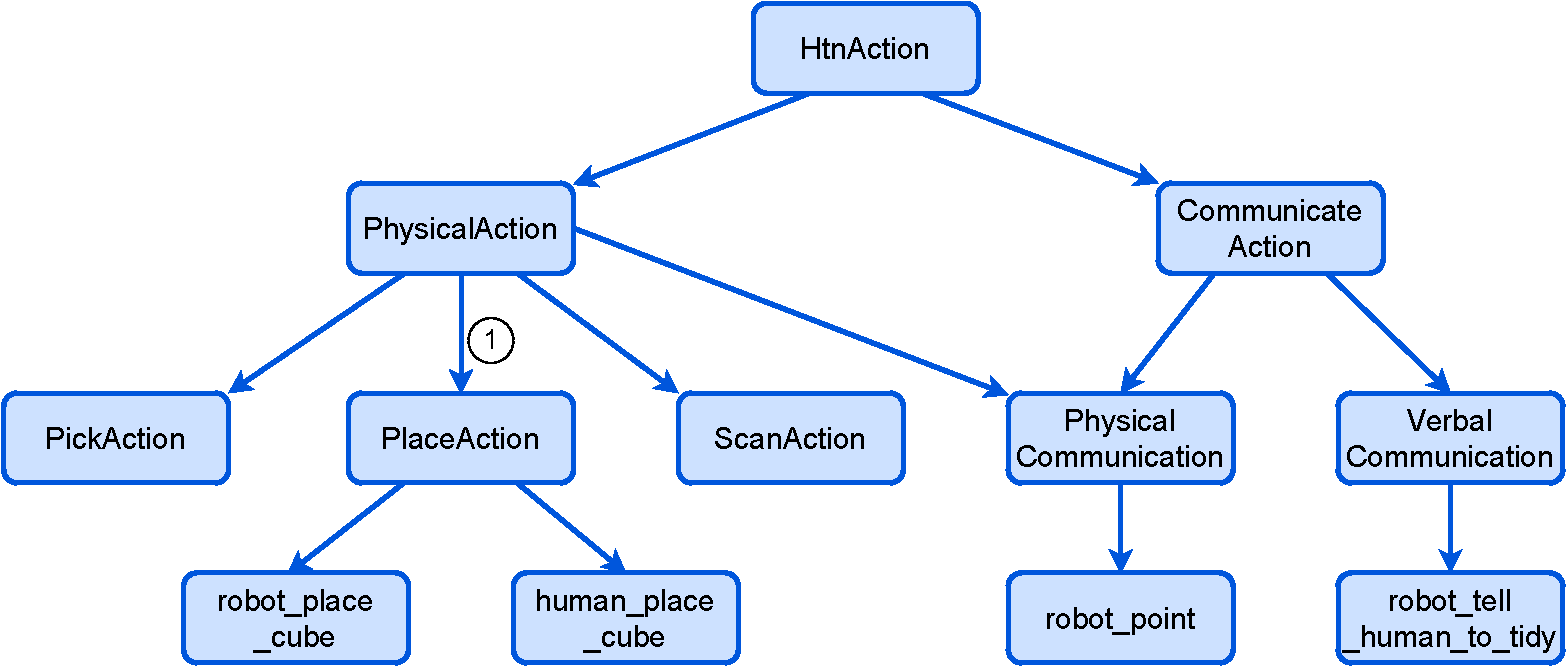
\includegraphics[width=\linewidth]{figures/chapter2/class_actions.pdf}
	\caption{The representation of an extract of the ontology class hierarchy graph of \acrshort{htn} actions. Taking the class PhysicalAction, the arrow \circledtext{1} has to be read	as \textit{``A DropAction is a kind of PhysicalAction''}.}
	\label{chap2:fig:class_actions}
\end{figure}

\begin{figure}[!ht]
	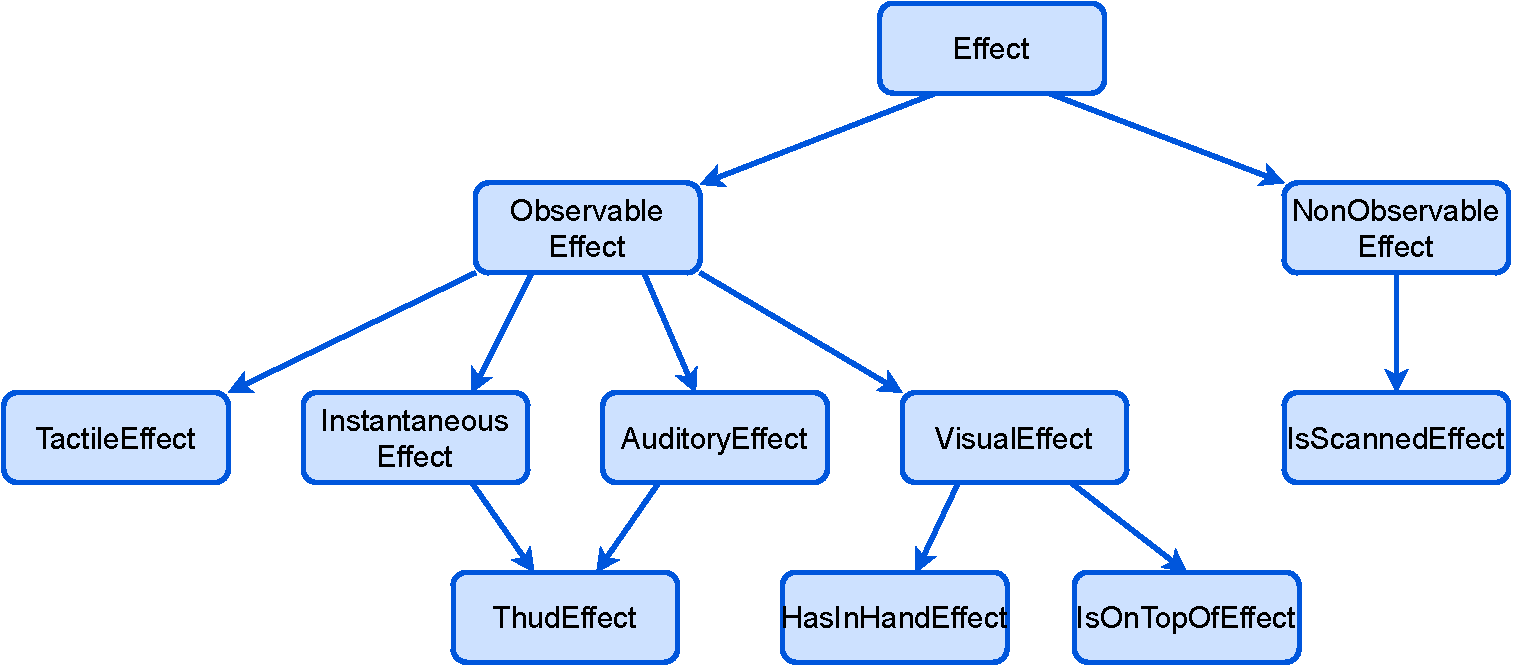
\includegraphics[width=\linewidth]{figures/chapter2/class_effects.pdf}
	\caption{The representation of an extract of the ontology class hierarchy graph of action effects. Taking the class ThudEffect, the arrows \circledtext{1} and \circledtext{2} indicate that ThudEffect is and an InstantaneousEffect and an AuditoryEffect.}
	\label{chap2:fig:class_effects}
\end{figure}

As we know, when an agent performs an action, the other agent may monitor it, in order to follow the task progress and to know when the action is over. A way to know that an action is over is to check if the action effects exist or not in the current worldstate. However, effects may be perceived differently according to the agent type as humans and robots does not have the same perception modalities (and even in one given type it can differ). In Figure~\ref{chap2:fig:class_effects}, we represented a possible way to model and classify action effects. And so, because Ontologenius is designed for \acrshort{hri}, it is possible to have different representations for robot agents and human agents. We present now a use case with its illustration in Figure~\ref{chap2:fig:kettle}. An agent may have to perform |HeatWaterInKettleAction|. If it is performed by the human, the robot has to monitor the action effects to know if the action is over or not. However, a robot is not able to observe that a kettle has finished to boil water, thus the action has a non-observable effect for the robot. Then, probably the robot will ask the human if the action is over or will see that the human performs its next action of the plan. Now, if we place ourselves in the case where the robot is the one performing the action -- with a smart kettle --, it wants to check if the human could be aware of the action end (because if they are not aware, it needs to communicate about it). The criteria \acrshort{jahrvis} takes into account is, was the effect observable by the human partner? To answer this question, it first needs to know what the observable effects of |HeatWaterInKettleAction| for the human (if there are). Then, it can query the human's belief base in Ontologenius and get the knowledge that for them, the effect of |HeatWaterInKettleAction| belongs to the class |ThudEffect| (when the kettle stops, it produces a thud) and |TactileEffect| (when the kettle boils water, it becomes hot).
	
\begin{figure}[!ht]
	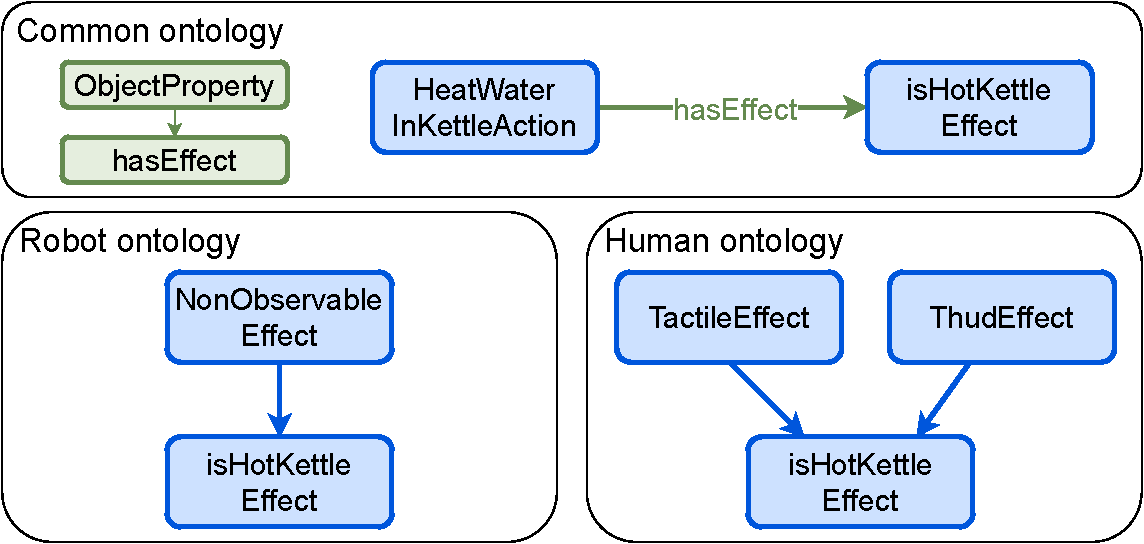
\includegraphics[width=\linewidth]{figures/chapter2/kettle.pdf}
	\caption{Illustration of the human and the robot having differing ontologies. Both have the common knowledge that HeatWaterInKettleAction has isHotKettleEffect as effect. However, in the robot ontology, isHotKettleEffect is defined as a NonObservableEffect whereas in the estimated human ontology it is defined as a TactileEffect and a ThudEffect which are both ObservableEffect as shown in Figure~\ref{chap2:fig:class_effects}.}
	\label{chap2:fig:kettle}
\end{figure}

Finally, as mentioned earlier and as visible in Listing~\ref{chap2:lst:classes}, Ontologenius allows to define label classes and so label for actions. These labels are then used by \acrshort{jahrvis} to communicate about the plan actions and based on a simple grammar we defined. For example, in ``\{Agent\} @Scan \{Pickable\}'', elements between braces are to be instantiated at execution time by \acrshort{jahrvis} communication process when needed. Then, the @ symbol indicates that the word is a verb that should be conjugated. Verb conjugations can also be found in the \acrshort{kb} as shown in Listing~\ref{chap2:lst:verb}. Thus, the communication manager could process it leading to ``I scanned the blue cube''.

\begin{lstlisting}[style=OwlTurtle, label={chap2:lst:verb}, caption={Description of the class describing the verb Drop in the third-person present-tense, in the OWL language using the Turle syntax.} ]
:DropTSPSimplePresent	rdf:type owl:Class ;
						rdfs:subClassOf :DropSimplePresent ;
						rdfs:subClassOf :ThirdSingularPersonalForm ;
						rdfs:label ``lâche''@fr ;
						rdfs:label ``drops''@en .
\end{lstlisting}

We have seen the possibilities offered by Ontologenius to \acrshort{jahrvis}. Now, we present the two internal action representations, one of the human actions in order to monitor them and the other one is of the robot actions, to allow the robot to monitor the human monitoring of its actions. 

\paragraph{Internal Action Representation}\label{chap2:par:act_rep}
What does \acrshort{jahrvis} need to monitor a human action? We defined a human action |Act| as: a predicate in the form of a triplet |ActPred| with its name |ActName|, the agent |AgentName| performing it and parameters |Params|; a list of preconditions |PrecondL|, a list of distinctive movements |MoveL| that the human could do when performing the action; a list of effects that we coined \textit{progression effects} |ProgEffectL| which are action effects, not enough to rule the action end but allowing the plan managers that an action is progressing towards its end; and a list of effects that we coined \textit{necessary effects} |NecessEffectL| which are action effects existing iff the action is over. Our action model takes the form of Jason beliefs written in an ASL file, added as input of the \acrshort{rja} Human Action Monitoring. A human action |Act| is represented as:
\begin{lstlisting}[style=aslDef]
actionModel(ActPred,PrecondL,MoveL,ProgEffectL,NecessEffectL).
\end{lstlisting}

\noindent
with |ActPred| being:
\begin{lstlisting}[style=aslDef]
			ActName(AgentName,Params).
\end{lstlisting}

For example, the action Place for a human is represented as:
\begin{lstlisting}[style=aslDef]
actionModel(place(Human,[Pickable,Support]),
			[hasInRightHand(Human,Pickable)],
			[rightHandMovingTowards(Human,SupportList)],
			[~hasInRightHand(Human,Pickable)],
			[isOnTopOf(Pickable,Support)]).
\end{lstlisting}

The choice to have two kinds of effects has been made in order to allow the Human Action Monitoring to be robust to a potentially unreliable perception. Indeed, for example in the case of a Place action, the perception of an object hold by a human can be jumpy, and receiving the fact that the object is not in the human's hand anymore. It could reappear a few instant later. On the other, if the robot perceives that the object has been placed on top of a support, it can assume that the action is really over. The algorithm of Human Action Monitoring will be more detailed in Section~\ref{chap2:subsec:h_moni}.

We designed a similar model for the robot actions but simpler as the preconditions are handle by the Motion Planner and the action progressing is followed through the ROS action client feedbacks. So, there is only the action triplet predicate and the necessary effects, which gives:
\begin{lstlisting}[style=aslDef]
			actionModel(ActPred,NecessEffectL).
\end{lstlisting}

For example, the action Place for a robot is represented as:
\begin{lstlisting}[style=aslDef]
actionModel(place(Robot,[Pickable,Support]),
				[~isHolding(Robot,Pickable), 
				isOnTopOf(Pickable,Support)]).
\end{lstlisting}

\subsubsection{Shared Plan Representation}\label{chap2:subsubsec:shared_p_rep}
As explained in Section~\ref{chap2:sec:levels}, we represent Shared Plans using \acrfull{htn}. This formalism allows to deal with goal-based and situation-based activities at different levels of hierarchy such as task, subtasks -- abstract tasks using planning vocabulary -- and actions -- atomic, primitive tasks -- and consequently to consider different levels of granularity. For example, it may be useful to \acrshort{jahrvis} to be able to request a plan for a given abstract task which failed\footnote{This is future work.}. Another advantage is that it is easy then for the robot to communicate about subtasks and not only about actions without context. However, according to the task or the domain, the \acrshort{htn} expressiveness for this matter raises discussion. Indeed, \acrshort{htn} plans often make use of recursive abstract tasks which becomes useless for replanning because such abstract tasks have no semantic meaning (\eg an abstract task called DropAllObjects can be decomposed into a primitive task DropObject and the abstract task DropAllObjects which is itself decomposed into DropObject and DropAllObjects, etc., in this case, to say that the abstract task DropAllObjects has failed does not give a useful information). 

Moreover, in the next section (see~\ref{chap2:subsec:feeding}), we show how \acrshort{jahrvis} feeds the episodic ontology, a timeline, with abstract and primitive task executions. It becomes humanly unreadable with recursive tasks. A concept such as the ``iterative task'' proposed by Martinie \etal{}~\cite{martinie_2011_structuring} would be interesting if used in a \acrshort{htn} plan for \acrshort{hri}. However, there is currently no such thing, so when manipulating such plans we have two modalities:
\begin{enumerate}
	\item the domain is written being aware of this issue and thus, \acrshort{jahrvis} takes abstract tasks as input besides primitive tasks (\ie in the current work, plans generated by \acrshort{hatpehda}\footnote{Based on domains intentionally written without recursive tasks by Guilhem Buisan.})
	\item the domain is written with recursive abstract tasks and thus, \acrshort{jahrvis} only selects primitive tasks as tasks being part of the plan (\ie in the current work, plans generated by \acrshort{hatp}\footnote{Reuse of domains written by Sandra Devin.})
\end{enumerate}

We define a shared plan as a sequence of primitive tasks having to be performed by an agent and, abstract tasks. An abstract is defined as follows: 
\begin{lstlisting}[style=aslDef]
	abstractTask(ID,State,Name,DecompoOf).
\end{lstlisting}
\noindent
where |ID| is an identification number proper to the given task, |State| is the task state estimation by the robot, |Name| is the name of the task and |DecompoOf| is the identification number (|ID|) of the abstract task that has been decomposed into other tasks, including the given task.
\noindent
And, a primitive task is defined as:
\begin{lstlisting}[style=aslDef]
	primTask(ID,State,Name,Agent,Params,Predecessors,DecompoOf).
\end{lstlisting}
\noindent
where |ID| is an identification number proper to the given task, |State| is the task state estimation by the robot, |Name| is the name of the task, |Agent| is the name of the agent that should perform the task, |Params| is the list of parameters required for the task execution, |Predecessors| is a list of task ids which correspond to tasks needing to be achieved before the given task can start, and |DecompoOf| is the ID of the abstract task that has been decomposed into other tasks, including the given task.

We defined nine possible values for a task |State|: |planned| (needs to be done later), |todo| (needs to be done now), |ongoing| (is in progress), |executed| (is achieved), |unplanned| (is not part of the plan anymore -- used with conditional plans (see Section~\ref{chap2:subsec:plan_handling})), |not_starting| (was to do but took to much time before starting), |not_finished| (started but has not been achieved), |not_seen| (executed but not observed by the other agent), |suspended| (needs to be set |unplanned|).

So, for example, an example of plan for a task where the robot gives instructions to the human in order to remove one cube from a shelf is:
\begin{lstlisting}[style=aslDef]
abstractTask(0, "planned", "tidy_cubes", (-1)). 
abstractTask(1, "planned", "tidy_one", 0). 
primTask(3, "planned", "robot_congratulate", 
		"robot", ["Helmet_2"], [8], 0).
primTask(4, "planned", "robot_tell_human_to_tidy", 
		"robot", ["cube_BBCG","Helmet_2","throw_box_green"], 
		[], 1).
abstractTask(5, "planned", "wait_for_human", 1).
abstractTask(6, "planned", "tidy", 0).
primTask(7, "planned", "human_pick_cube",
		"Helmet_2", ["cube_BBCG"], [4], 6).
primTask(8, "planned", "human_drop_cube", 
		"Helmet_2", ["throw_box_green"], [9], 6).
primTask(9, "planned", "robot_wait_for_human_to_tidy", 
		"robot", [], [7], 5).
primTask(11, "planned", "idle", "Helmet_2", [], [3], 0).
\end{lstlisting}

\subsubsection{Feeding the Knowledge Base}\label{chap2:subsec:feeding}
Until know, we stayed focused on semantic knowledge going from the external \acrshort{kb} to \acrshort{jahrvis}. But, as mentioned earlier, one of the external \acrshort{kb} is dedicated to episodic knowledge. This \acrshort{kb} takes the form of a timeline, managed by Mementar. Whereas Ontologius feeds \acrshort{jahrvis} with knowledge, the flow is inverted for the episodic data, as Mementar is fed by \acrshort{jahrvis} among other components. Indeed, when an abstract or primitive task is started or achieved, this information is sent to Mementar for storage with the associated ID and time stamp. The objective is to have a history of the task proceeding. One of the possible use of such a history is for the robot to refer to past events during a task when communicating. We illustrate the timeline in Figure~\ref{chap2:fig:timeline} with the same example as the one above for the plan, one cube had to be removed by the human.

\begin{figure}[!ht]
	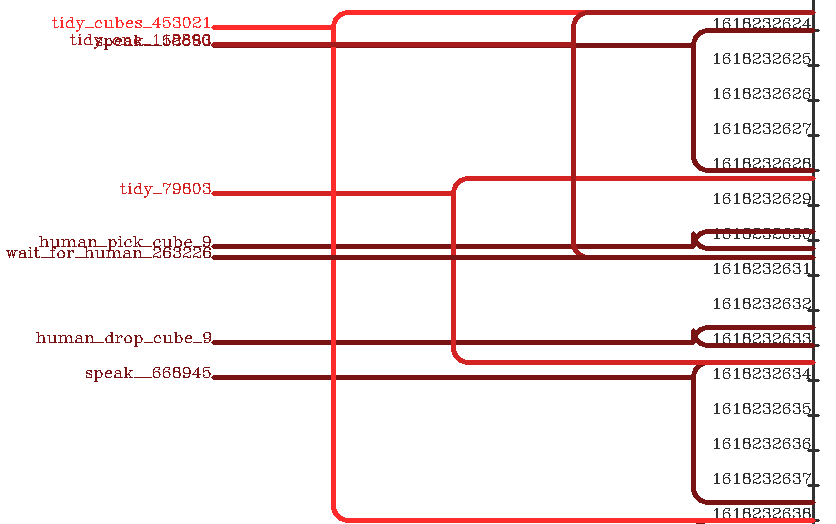
\includegraphics[width=\linewidth]{figures/chapter2/timeline.png}
	\caption{Example of timeline a task where one cube had to be removed from the shelf by the human. It has been automatically generated by Mementar after having received data from \acrshort{jahrvis}.}
	\label{chap2:fig:timeline}
\end{figure}

Moreover, \acrshort{jahrvis} adds the semantic data associated to a task -- agent and parameters -- to the semantic ontology.

\subsection{Interaction Session Management} \todo{mettre state machine théorique que j'ai faite ? je n'ai pas redeveloppé ce module depuis mummer}
This process handles the interaction sessions. An interaction session is triggered when a human is close enough to start a conversation and seems willing to, \ie when the fact  \fact{isEngagedWith}{human\_i}{robot} is added to the knowledge base and sent to \acrshort{jahrvis}. In this way, the robot tries to respect people that does not want to interact with it. From there, the robot is in the first phase of the interaction session, the \textit{greetings}. The robot says hello to the human and announces the activities it can perform with them, depending on the context they are in. The interaction manager triggers the tracking of the human's head by the robot head. This has two purposes: to signal the robot's engagement and to monitor the human's actions. This behavior is quite similar to the one described by Satake \etal~\cite{satake_2015_should}. 

An interaction session stays open as long as the human and the robot perform activities together, \ie as long as the human is engaged in the interaction. This engagement is monitored by the robot in different ways: through the predicate \fact{isEngagedWith}{human\_i}{robot} during dialogue phases outside a task and through what is happening during a task. If at some point the human is not perceived for a while or the human says goodbye, then the manager ends the session. In the latter case, the robot replies with goodbyes. Finally, it returns to its home-base if it has one.


\subsection{Human Actions Monitoring}\label{chap2:subsec:h_moni}\todo{attention utilisation de monitoring ou recognition ?? monitoring plutôt pour le handling de la tête du robot non ?}
In order to coordinate properly, humans monitor each others when they are in a joint action (see Section~\ref{chap1:subsubsec:monitoring}). The robot needs the same kind of process to be able to assess if the human is doing the action of the plan it expects or not. Existing solutions exist to monitor or recognize human actions but none of them matched all our criteria which are: \todo{faire un état de l'art rapide}
\begin{bulletList}
	\item it should be easy and quick to add a new action that the robot can monitor
	\item the process should output the action parameters
	\item the process should give information about the action progress, \ie model the action start and progression when possible and not only the end
	\item it needs to be robust to a potentially unreliable perception
	\item an available open-source code 
\end{bulletList}

Thus, we implemented our own model-based solution with an \acrshort{rja} dedicated to \acrfull{ham}. It relies on the action model presented in Section~\ref{chap2:par:act_rep} which it loads at initiation. We chose to base our action monitoring process on human movements and action effects that the robot can observe. As it needs to monitor them, it extracts the predicate types corresponding to those and subscribes to updates about these facts to Ontologenius as explained in Section~\ref{chap2:subsec:know}. 

Continuously, the \acrshort{ham} \acrshort{rja} monitors facts and human movements that are present in the action model, and sends to the \acrfull{hpm} \acrshort{rja} three types of lists of facts: 
\begin{bulletList}
	\item list of actions that may have started that we coined \emph{possibly started actions}
	\item list of actions that may be progressing that we coined \emph{possibly progressing actions}
	\item list of actions that are estimated as finished that we coined \emph{possibly achieved actions} 
\end{bulletList}

Action states are updated according to received facts. When the state of an action changed to \emph{possibly started}, \emph{possibly progressing} or \emph{possibly achieved}, the affected list is updated and sent to the \acrshort{hpm}. 

The algorithm we developed can be depicted in the form of a Finite State Machine representing the state of one action as shown in Figure~\ref{chap2:fig:action_monitoring} and is implemented in ASL (the code is available in Appendix~\ref{app:jahrvis:h_monitoring}). Each transition is triggered by the addition or the deletion of a fact. Using Jason rules -- they are quite similar to Prolog rules, facts are analyzed to see if they match a movement or an effect of a known action. For example, if we look at the Place action example presented in Section~\ref{chap2:par:act_rep}, it expects the fact \fact{rightHandMovingTowards}{Human}{Support} as a movement. Therefore, receiving \fact{rightHandMovingTowards}{human\_4}{table\_2} will match a Place action movement, however, receiving \fact{rightHandMovingTowards}{human\_4}{milk\_bottle\_2} will not, as the milk\_bottle\_2 does not belong to the Support class (but this fact may be useful for monitoring another action).
 
It is not shown on the Figure for clarity reasons, but each state, except Possibly achieved, has a transition to the final state which is triggered by a timeout. Currently, this timeout is the same for each action but as every action type might be of different lasting, a timeout could be specifically set for each one. All the other transitions of the state machine are described in Table~\ref{chap2:tab:action_monitoring}. 
 
\begin{figure}[!ht]
	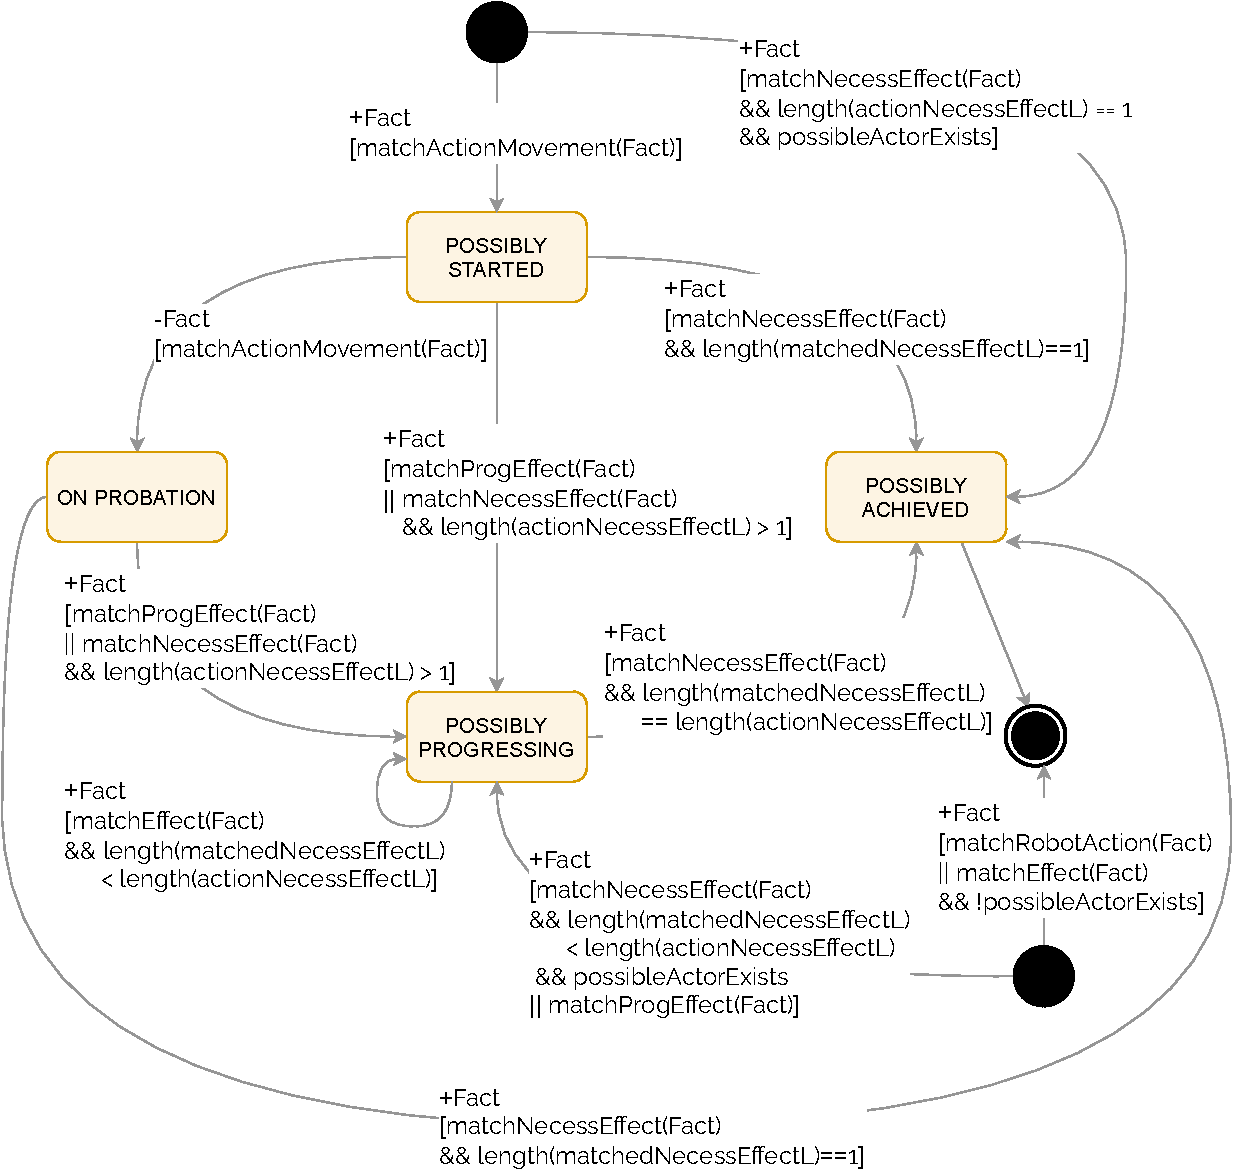
\includegraphics[width=\linewidth]{figures/chapter2/action_sm.pdf}
	\caption{Representation of the \acrfull{ham} \acrshort{rja} in the form of a Finite State Machine representing the state of one action.}
	\label{chap2:fig:action_monitoring}
\end{figure}

\newgeometry{left=1.5in,right=1.3in,top=1.1in,bottom=0.5in,includefoot,includehead,headheight=13.6pt}
\begin{landscape}
	\vspace*{\fill}
	\begin{table}[htb!]
	\caption{Description of the Finite State Machine shown in Figure~\ref{chap2:fig:action_monitoring}.}
	\label{chap2:tab:action_monitoring}
	\begin{tabularx}{\linewidth}{| c | c | c | X |}
		Current State & Input and Condition & Next State & Explanation\\ 
		\hline \hline
	\multirow{4}{*}{Initial State}  & +Fact [matchActionMovement(Fact)] & Possibly Started & When a fact matching a movement for a given action is received, \acrshort{ham} computes that the human may have initiated an action\\  
		\cline{2-4}
		&  \makecell{+Fact [matchNecessEffect(Fact) 
			\\ \&\& length(actionNecessEffectL)	== 1
			\\ \&\& possibleActorExists]} & Possibly Achieved & The robot may have missed the movement or the progression effect of an action because it was not looking or the perception did not detect it. Then when a necessary effect is received and that only one exists for the action, the action is estimated as achieved if it is possible to find an agent who may have performed it.\\  
		\cline{2-4}
		&  \makecell{+Fact [matchNecessEffect(Fact) 
		\\ \&\& length(matchedNecessEffectL)
		\\ < length(actionNecessEffectL)
		\\ \&\& possibleActorExists
		\\ || matchProgEffect(Fact)]} & Possibly Progressing & Similarly to the case above, the robot may have missed the movement or the progression effect of an action. However, if this action has several necessary effects, the action is considered as progressing.\\  
		\cline{2-4}
		& \makecell{+Fact [matchRobotAction(Fact)
		\\ || matchEffect(Fact) \&\& !possibleActorExists]} & Final State & The \acrshort{ham} is aware of the actions executing by the robot so it does not mismatched its action effects with the ones of another agent. If an effect matches, nothing happen. Likewise if an effect is detected but no agent could be found that might have done it.\\  
		\hline 
	\end{tabularx}
\end{table}
\vspace*{\fill}
 \begin{table}[htb!]
 	\caption*{Table~\ref{chap2:tab:action_monitoring}: (continued)}
	\begin{tabularx}{\linewidth}{| c | c | c | X |}
		Current State & Input and Condition & Next State & Explanation\\ 
		\hline \hline
		\multirow{3}{*}{Possibly Started}  
		& \makecell{+Fact [matchProgEffect(Fact)
			\\ || matchNecessEffect(Fact) 
			\\ \&\& length(actionNecessEffectL) > 1]} & Possibly Progressing & When a fact corresponding to a progression effect of the started action is received, or it matches a necessary effect but there are more than one for this action, \acrshort{ham} reinforces its estimation that this action is ongoing by setting it to the progressing state.\\  
		\cline{2-4}
		& \makecell{+Fact [matchNecessEffect(Fact) 
			\\ \&\& length(matchedNecessEffectL) == 1]} & Possibly Achieved 
		& When a fact corresponding to a necessary effect is received and that there is only one for the started action, the action is considered as achieved as the robot is able to observe its effect and that it had observed the human starting it.\\  
		\cline{2-4}
		& -Fact	[matchActionMovement(Fact)] & On Probation & When a movement fact is removed from the belief base without having observed an effect, it might mean that it was a false estimation and that the action is not starting. However, it might also be the robot perception being sporadic and so the action goes in this temporary state waiting for a potential coming effect.\\  
		\hline
	\end{tabularx}
\end{table}
\vspace*{\fill}
  \begin{table}[htb!]
  	\caption*{Table~\ref{chap2:tab:action_monitoring}: (continued)}
	\begin{tabularx}{\linewidth}{| c | c | c | X |}
		Current State & Input and Condition & Next State & Explanation\\ 
		\hline \hline
		\multirow{2}{*}{On Probation} 
		& \makecell{+Fact [matchProgEffect(Fact)
			\\ || matchNecessEffect(Fact)
			\\ \&\& length(actionNecessEffectL) > 1]} & Possibly Progressing & An effect is detected and the action state is resumed.\\
		\cline{2-4}
		& \makecell{+Fact [matchNecessEffect(Fact) 
			\\ \&\& length(matchedNecessEffectL) == 1]} & Possibly Achieved 
		& A necessary effect is detected and as there is only one for this action, it is considered as achieved.\\
		\hline
		\multirow{2}{*}{Possibly Progressing} 
		& \makecell{+Fact [matchNecessEffect(Fact) 
			\\ \&\& length(matchedNecessEffectL)
			\\ == length(actionNecessEffectL)]} & Possibly Achieved 
		& An necessary effect is received and in total, for this action, there was as many necessary effects received as the ones defined for this action.\\
		\cline{2-4}
		& \makecell{+Fact [matchEffect(Fact) 
			\\ \&\& length(matchedNecessEffectL)
			\\ < length(actionNecessEffectL)]} & Possibly Progressing 
		& When an action effect is received and that either it is another progressing or not the last necessary effect expected for the action, the action state remains progressing.\\  
		\hline
		Possibly Achieved & -- & Final State & When an action is estimated as achieved, this is its final state.\\
		\hline
	\end{tabularx}
	
\end{table}
\vspace*{\fill}
\end{landscape}
\restoregeometry

When the software starts, the \acrshort{ham} extracts from the internal action representation presented in Section~\ref{chap2:subsubsec:action_rep}, all the types of facts that should be monitored. Then, it queries Ontologenius to send it each updates about these facts. Thus, when the robot designers decide that a new action should be recognized by the robot, the only thing to add is the action model in \acrshort{jahrvis} belief base.

Moreover, sometimes new facts are actually effects of robot actions. In order to avoid that robot actions are mistaken for human ones, the \acrfull{aem} warns the \acrshort{ham} when the robot executes an action. 

Finally, all the functions to check if a new fact update matches an action effect are Jason rules. They rely on Ontologenius as there is a need to compare the predicate object and subject expected classes of an action effect with the received ones.

\subsection{Shared Plans Handling}\label{chap2:subsec:plan_handling}
In order to correctly perform collaborative tasks with humans, the robot needs to know how to do them. One way is to have a planner with a domain, computing a plan at execution time based on its current knowledge about the environment and interaction. Then, the robot must be endowed with a way to manage the execution of this recipe. As we place ourselves in the context of joint action, plans manipulated by the robot are shared plans, as presented in Section~\ref{chap2:subsubsec:shared_p_rep} (to differentiate from the ASL plans presented in Section~\ref{chap2:subsec:jason} which code all the \acrshort{rja}).

We claim that the robot ability to handle and execute shared plan is enhanced when endowed with \acrfull{tom} (see Sections~\ref{chap1:subsec:tom} and~\ref{chap1:subsec:tom_hri}), as shown by Devin~\cite{devin_2016_implemented}. It allows the robot to be aware of false beliefs or belief divergences in the human's point of view. When such things happen, it can react appropriately, either by acting or communicating. We gave the robot such an ability\footnote{The robot has a first-order \acrshort{tom}, it estimates the human knowledge about the task but it does not compute what the human thinks of the robot knowledge about the task (second-order \acrshort{tom})}, \textit{via} two processes: the \acrfull{rpm} and the \acrfull{hpm} (see Figure~\ref{chap2:fig:sup_overview}). Therefore, the first one handles the robot's beliefs about the plan and the action execution while the second handles the human's beliefs about the plan and the communication with the human. The \acrshort{rja}s implementing these processes are presented in Sections~\ref{chap2:subsubsec:robot_plan} and~\ref{chap2:subsubsec:human_plan}.

As we designed \acrshort{jahrvis} to be as generic as possible, it can manage different kinds of human-robot shared plans as input: (1) classical shared plans, (2) shared plans for which actions might not be allocated to an agent at planning time and objects might be referred to with a semantic query, and (3) conditional shared plans which anticipate different possibilities for the human decision/action. What we call classical shared plans are as the ones returned by \acrfull{hatp}~\cite{lallement_2014_hatp}. 

The second type of shared plans is an extension of the work of Devin about postponing some decisions from planning time to execution time about the actor of some actions and some parameters~\cite{devin_2017_decisions}. In works previous to Devin, all the actions\footnote{We use the term action interchangeably with primitive task in this section.} of the computed plans were
allocated and completely instantiated during plan elaboration. For example, the first action of the shared plan for a blocks building task could be: 
\begin{lstlisting}[style=inline]
primTask(7, "planned", "pick_place_cube", "robot", 
["red_cube_1", "placement_1"], [4], 6).
\end{lstlisting}
We re-implemented her idea of \emph{Agent X} in our plan managers (with some modifications, for example we do not replan once an action is allocated), enabling the choice of the agent who should perform the action at execution time when the planner has computed that both agents could do it. So we can have the planner returning:
\begin{lstlisting}[style=inline]
primTask(7, "planned", "pick_place_cube", "AgentX", 
["red_cube_1", "placement_1"], [4], 6).
\end{lstlisting} 
In this case, according to what the robot estimates the human wants to do, the robot can allocate the action to itself or to them. Moreover, she introduced the use of the notion of object similarity: two similar objects will have the same role in the task. With this modification, the first action of the shared plan becomes
\begin{lstlisting}[style=inline]
primTask(7, "planned", "pick_place_cube", "robot", 
["red_cube", "placement"], [4], 6).
\\ with red_cube beeing a generic type an not an individual
\end{lstlisting}
To have more expressiveness, we brought a new modification to the plan returned by \acrshort{hatp}, in collaboration with Guillaume Sarthou. Indeed, instead of returning an object generic name, it returns a \sparql{} query with the constraints used in the domain. Thus, keeping the same example as previously, the action becomes
\begin{lstlisting}[style=inline]
primTask(7, "planned", "pick_place_cube", "robot", 
["?0 isA Cube. ?0 hasColor red. ?0 isReachableBy ?1 
NOT EXISTS { ?0 isOnTopOf ?2. ?2 isA Cube }", 
"placement"], [4], 6).
\end{lstlisting}
This allows the \acrshort{rpm} to directly request Ontologenius to get an object list matching this query and to choose among it at execution time. And, when the human performs an action with a \sparql{} query as parameter, the \acrshort{hpm} can check if the object on which the human is acting matches the query. We can see that this solution brings precision compared to the one presented by Devin. Indeed, |"red_cube"| does not tell that it should be reachable by an agent and that it should not be on the top of another cube yet but |"?0 isA Cube. ?0 hasColor red. ?0 isReachableBy ?1| |NOT EXISTS { ?0 isOnTopOf ?2. ?2 isA Cube }"| does. For example, in Devin, the reachability test was added to the plan manager of the supervisor which is task specific. 

\begin{figure}[!htb]]
	\centering
	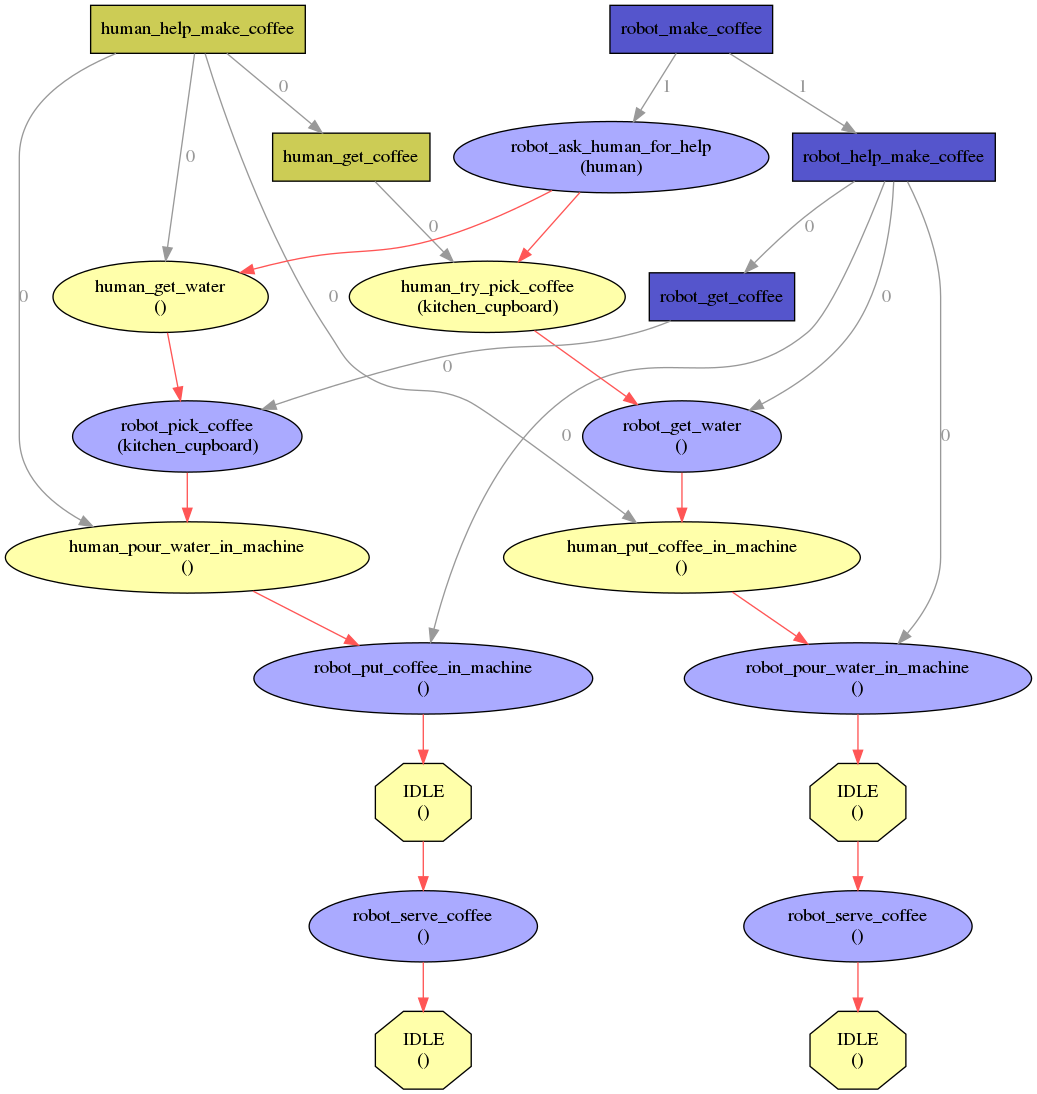
\includegraphics[width=\linewidth]{figures/chapter2/cond_plan_coffee.png}
	\caption{A conditional plan computed by \acrshort{hatpehda}, a planner developed by Guilhem Buisan who also wrote the domain which served for this plan. The ellipses correspond to primitive tasks while rectangles represent abstract ones. The octagons represent the default actions (\textit{IDLE} and \textit{WAIT}). The blue shapes are robot tasks and the yellow ones are the human ones. Finally, red arrows indicate the sequence of actions in the plans and gray ones represent hierarchical links, \textit{i.e.}~the links between the tasks as defined in the \acrshortpl{htn}. The plan indicates that the robot has to ask for human help. Then, the human will either get the coffee or fill the water. Thus, at planning time, the choice of human actions is not made, but thanks to the conditional plan, both possible solutions are planned and it is up to \acrshort{jahrvis} to follow the proper one depending on the human action detected during execution.}
	\label{chap2:fig:cond_plan_coffee}
\end{figure}

Finally, the last type of shared plans we manipulated is conditional plan, generated by \acrfull{hatpehda}~\cite{buisan_2021_human}. It is another mean to postpone decision at execution time about an agent actor or parameters, with plans where branch junctions concern human decision. For example, in Figure~\ref{chap2:fig:cond_plan_coffee}, is shown a conditional plan computed by \acrshort{hatpehda}. The plan indicates that the robot has to ask for human help. Then, the human will either get the coffee or fill the water. Thus, at planning time, the choice of human actions is not made, but thanks to the conditional plan, both possible solutions are planned and it is up to \acrshort{jahrvis} to follow the proper one depending on the human action detected during execution.

\acrshort{jahrvis} could be used to execute plans from other \acrshort{htn} planners than \acrshort{hatp} and \acrshort{hatpehda} by adding a Java class to format abstract and primitive tasks as presented in Section~\ref{chap2:subsubsec:action_rep} -- \acrshort{hatp} and \acrshort{hatpehda} have a dedicated Java class each, for action formatting, but their plans are handled with the same code in the plan managers.

Now, we will present the two processes in charge of the shared plan management, one to handle the plan on the robot side, \ie its updates and the action execution, and the other one to handle the estimated human mental states about the shared plan. When either the robot or the human starts and finishes an action execution, facts corresponding to these events, are added to Ontologenius and Mementar to keep track of what happened during the interaction. It also registers the data about the abstract task. Then, a component of the robotic architecture used to generate communication about elements, the \acrfull{reg}, can use such information when querying by \acrshort{jahrvis} to refer to the past (\eg ``the cube you took'').

When we will mention the robot monitoring with its head, it is done through a component described in Section~\ref{chap2:par:act_rep}.

\todo{replan,contingencies?}

\subsubsection{Robot Plan Management}\label{chap2:subsubsec:robot_plan}

As explained earlier, there are two processes to manage the shared plans. One of them is the \acrfull{rpm}. It is in charge of the plan updates, maintaining the robot knowledge about the ongoing goal, and deciding which action should be performed by the robot and when. 

When it receives a new goal from the \acrlong{ism}, it queries the Task Planner for a plan. This plan is a sequence of abstract and primitive tasks as described in Section~\ref{chap2:subsubsec:shared_p_rep}. First, when receiving the plan, and then at each end of action execution, the abstract and primitive task states of the plan are screened in order to find the next primitive task to perform. The found ones have their state set to |todo|. The implemented algorithm to do so is presented in Algorithm~\ref{chap2:algo:UP}. 

\begin{algorithm}[!htb]
	\caption{Update of a plan}
	\label{chap2:algo:UP}
	\begin{algorithmic}
		\Function{UpdatePlan}{}
		\ForEach{primTask($i$,$state_i$,$preds_i$,$decompoOf_i$),\\\hfill $state_i=$ \algConst{PLANNED}$,i \in \mathbb{N}$}{planPrimTasks}
		\State $preds$ $\coloneqq$\textsc{FindAll}($j$) 
		\\\hfill such as primTask($j$,$state_j$,$preds_j$,$decompoOf_i$) $\in$ planPrimTasks,\\ \hfill $j \in preds_i$, $state_j$ $\neq$ \algConst{EXECUTED}
		\If{$preds = \emptyset$}
		\State primTask($i$,\algConst{PLANNED},$preds_i$,$decompoOf_i$) 
		\\\hfill $\coloneqq$ primTask($i$,\algConst{TODO},$preds_i$,$decompoOf_i$)
		\State \textsc{UpdateAbstractTasksToOngoing($decompoOf_i$)}
		\EndIf
		\EndFor
		\If{$\forall$ primTask($state$) $\in$ planPrimTasks, 
			\\\hfill $state=$ \algConst{EXECUTED} or $state=$\algConst{UNPLANNED}}
		\State Goal(\algConst{ONGOING}) $\coloneqq$ Goal(\algConst{SUCCEEDED})
		\EndIf
		\EndFunction
		\Statex
		\Function{UpdateAbstractTasksToOngoing}{$i$}
		\If{$\exists$ abstractTask($i$,$state$,$decompoOf$) and $state=$ \algConst{PLANNED}}
		\State abstractTask($i$,\algConst{PLANNED},$decompoOf$) $\coloneqq$ abstractTask($i$,\algConst{ONGOING},$decompoOf$)
		\State \textsc{UpdateAbstractTasksToOngoing($decompoOf$)}
		\EndIf
		\EndFunction
	\end{algorithmic}
\end{algorithm}

As we used Jason, a process can react to events (see Section~\ref{chap2:subsec:jason}). Every abstract or primitive task state update triggers an event. We represented what happened when a primitive task is updated to |todo| in Algorithm~\ref{chap2:algo:todo}. There are three possible cases, either an action is to be performed by the human, or the robot, or it is undefined which is represented by the AgentX. 

When an action should be performed by the human and if the robot does not have an action to do at the same time, the robot has to monitor them, or rather the parameters of their action, in order to be aware of what they are doing. To monitor, robot can use several modalities when they exist. Indeed, it can monitor with the camera on its head but also with a (lidar) scanner for example. As the most important thing for the \acrshort{rpm} is to monitor parameters and not how to monitor them, it sends to a component in charge of the robot resources the objects of interest for the given action. For now, only one parameter among the parameter list is selected to be monitored. The function to select this object of interest among the action parameters is simple, we take the first of the list, but it could be refined. Or, as explained earlier, parameters can be in the form of \sparql{} queries. If it is the case, the robot chose to monitor the human closest one among the ones returned by Ontologenius. Then, it waits an update on the action state -- which is updated by the \acrfull{hpm} and then sent to the \acrshort{rpm}.


\begin{algorithm}[!htb]
	\caption{Event action todo in \acrshort{rpm}}
	\label{chap2:algo:todo}
	\begin{algorithmic}
	\Function{On}{primTask($i$,\algConst{TODO},$name$,$agent$,$params$)}
	\If{$agent \in$ Human and $name \in$ PhysicalAction}
	\State $p \coloneqq$ \textsc{ChooseObjectToMonitor($params$)}
	\State \textsc{SetMonitorObject($p$)}
	\State \textsc{WaitForPrimTaskStateToChange($i$)}
	\ElsIf{$agent \in$ Robot or $agent \in$ AgentX}
		\If{$\exists p \in params, p$ is a \sparql{} query}
		\State $electedAgent,newParams\coloneqq$
		\\\hfill \textsc{InstantiateParams}(primTask($i$,$state$,$name$,$agent$,$params$))
		\State $params \coloneqq newParams$
		\EndIf
		\If{$electedAgent \neq \varnothing$}
			\State primTask($i$,\algConst{TODO},$name$,$agent$,$params$) 
			\\\hfill $\coloneqq$ primTask($i$,\algConst{TODO},$agents[0]$,$params$)\Comment{Triggers a new \textsc{On} function}
		\Else
			\State \textsc{AllocatePrimTask}(primTask($i$,$state$,$name$,$agent$,$params$))
			\If{$agent \notin$ Human}
			 \State \textsc{SendMessage}(ActionExecutionManager,primTask($i$,$name$,$agent$,$params$))
			 \EndIf
		\EndIf
	\EndIf
	\EndFunction
	\Statex
	\Function{InstantiateParams}{primTask($i$,$state$,$name$,$agent$,$params$)}
	\ForEach{$p$}{$params$}
	\If{$p$ is a \sparql{} query}
		\State $sparqlQ \coloneqq$ \textsc{SparqlToElementList($p$)} \Comment{$sparqlQ$ is a list of list. }
		\State $electedAgent = \varnothing$
		\If{$\exists a_i \in sparqlQ, a_i \in $Agent and  $a_i$ is unique}
			\State $electedAgent \coloneqq a_i$
		\EndIf
		\State add $sparqlQ$ in $newParams$
	\Else
		\State add $p$ in $newParams$
	\EndIf
	\EndFor
	\State \Return $electedAgent,newParams$
	\EndFunction
	\algstore{todo}
\end{algorithmic}
\end{algorithm}

When an action should be performed by the robot or the AgentX, first it needs to check if all action parameters are already instantiated and not a \sparql{} request. When a parameter is a \sparql{} request, it queries Ontologenius to get all the objects matching it, and eventually, the agents, in the form of a list of list. For example, if the \sparql{} request is |?0 isA Cube. ?0 hasColor green|, then the result could be |[[cube\_1],[cube\_2]]|. Or, in case where there is another element in addition to the object, such as an agent, \eg |?0 isA Cube. ?0 hasColor green. ?0 isReachableBy ?1|, the result could be |[[cube\_1,robot],[cube\_2,human]]|. Sometimes, an agent action is allocated to the AgentX but the environment may have changed since planning time. Then, there may be one agent only, either the human or the robot, returned in the object list. In this case, the agent action value is updated with this agent. Next, the action has to be allocated to an agent. If the agent value corresponds to the robot, the only thing to do is to select the parameters to execute the action in case some of them are object list. For now the function is simple, the robot choses the first one of the list. If the agent value corresponds to the AgentX, then the \acrshort{rpm} checks if another action exists with the same parameters and the |todo| state. Indeed, the human cannot perform two actions at the same time so the \acrshort{rpm} can allocated one to the robot. In case there is no other action, as we think the robot as a human helper, it should leave the choice to them if they want to perform the action or not. Devin showed that naive users preferred when the robot asked them what they wanted to do~\cite{devin_2017_decisions} but it has been shown that regular users preferred when a robot adapted to them\todo{add ref}. Therefore, we chose the adaptive option, where the robot waits a few seconds to see if the human starts to perform the action. If they do, the action is allocated to the human and if they do not, the \acrshort{rpm} allocates the action to the robot. Finally, when an action was allocated to the robot, it is sent to the \acrlong{aem} that will handle the action execution as indicated by its name.

\begin{algorithm}[!htb]
	\ContinuedFloat
	\caption{Event action todo in \acrshort{rpm}(continued)}
	\begin{algorithmic}
	\algrestore{todo}
	\Function{AllocatePrimTask}{primTask($i$,$state$,$name$,$agent$,$params$)}
		\If{$agent \in $Robot or 
			\\\hfill $\exists$ primTask($j$,$state$,$name$,$agent$,$params$), $state=$ \algConst{TODO}, $j \neq i$,$agent \in$ AgentX)} 
			\State \textsc{AllocatePrimTaskToRobot($i$,\algConst{TODO},$name$,$agent$,$params$)}
		\Else
			\While{$t_{current} < T_{max\_wait}$ or  (($state=$\algConst{ONGOING} or $state=$\algConst{EXECUTED}) \\\hfill and $agent \in$ Human)}\\\Comment{The Human Plan Manager can send a message to update the status of primTask($i$)}
			\EndWhile
			\If{$agent \notin$ Human}
				\State \textsc{AllocatePrimTaskToRobot($i$,\algConst{TODO},$name$,$agent$,$params$)}
			\EndIf
		\EndIf
	\EndFunction
	\Statex
	\Function{AllocatePrimTaskToRobot}{$i$,$state$,$name$,$agent$,$params$}
	\ForEach{$p$}{$params$}
		\State \textsc{SelectParams($params$)}
		\State primTask($i$,\algConst{TODO},$name$,$agent$,$params$) 
		\\\hfill $\coloneqq$ primTask($i$,\algConst{TODO},robot,$params$)
	\EndFor
	\EndFunction
	\end{algorithmic}
\end{algorithm}


We represented what happened when a primitive task is updated to |executed| in Algorithm~\ref{chap2:algo:executed}. As explained above, the manipulated plans can be conditional plans. Thus, at the end of each action execution, the \acrshort{rpm} looks for if actions of other branches exist. First, it tries to find if the agent and predecessors of the action which just finished are the same than the one another action. If it is the case, all the abstract and primitive task descendant of this found action are set |unplanned|. 

\begin{algorithm}[!htb]
	\caption{Event action executed in \acrshort{rpm}}
	\label{chap2:algo:executed}
	\begin{algorithmic}
	\Function{On}{primTask($i$,\algConst{EXECUTED},$name$,$agent$,$params$,$preds$,$decompoOf$)}
		\State \textsc{EndObjectMonitoring($params$)}
		\State \textsc{RemoveParallelBranches($agent$,$preds$)}
		\State \textsc{UpdateAbstractTasksToExecuted($decompoOf$,\algConst{EXECUTED})}
		\State \textsc{UpdatePlan} \Comment{see Algorithm~\ref{chap2:algo:UP}}
	\EndFunction
	\Statex
	\Function{RemoveParallelBranches}{$agent$,$preds$}
		\State $primTasksToUnplan \coloneqq$ \textsc{FindAll}(primTask) 
		\\\hfill with same $agent$ and $preds$, and ($state=$\algConst{TODO} or $state=$\algConst{SUSPENDED}) 
		\State \textsc{removePrimTasks}($primTasksToUnplan$)
	\EndFunction
	\Statex
	\Function{removePrimTasks}{$primTasksToUnplan$}
		\ForEach{primTask}{$primTasksToUnplan$}
			\State primTask($i$,$state$,$name$,$agent$,$params$,$preds$,$decompoOf$) 
			\\\hfill $\coloneqq$ primTask($i$,\algConst{UNPLANNED},$name$,$agent$,$params$,$preds$,$decompoOf$)
			\State \textsc{UpdateAbstractTasksToExecuted($decompoOf$,\algConst{UNPLANNED})}
			\State \textsc{RemoveChild($i$)}
		\EndFor
	\EndFunction
	\Statex
	\Function{RemoveChild}{$i$}
		\State $primTasksToUnplan \coloneqq$ \textsc{FindAll}(primTask($j$)) where $i \in preds_j$ 
		\State \textsc{RemovePrimTasks}($primTasksToUnplan$)
	\EndFunction
	\Statex
	\Function{UpdateAbstractTasksToExecuted}{$i$,$stateToSet$}
		\If{$\exists$ (abstractTask($i$,$state$,$decompoOf$) or  primTask($i$,$state$,$decompoOf$)) and 
			\\\hfill ($state=$ \algConst{EXECUTED} or $state=$ \algConst{UNPLANNED})}
			\State abstractTask($i$,\algConst{PLANNED},$decompoOf$) $\coloneqq$ abstractTask($i$,$stateToSet$,$decompoOf$)
			\State \textsc{UpdateAbstractTasksToExecuted($decompoOf$,$stateToSet$)}
		\EndIf
	\EndFunction	
	\end{algorithmic}
\end{algorithm}		

\clearpage
\subsubsection{Human Plan Management}\label{chap2:subsubsec:human_plan}\todo{add wait and check already performed (state based + transition based)}
The \acrfull{hpm} keeps track of the estimated human mental state about the ongoing shared plan, endowing the robot with \acrlong{tom} (see Section~\ref{chap1:subsec:tom}). The role of this process is central, as it receives the data about the human action monitoring, it deduces what the human might or might not know about the plan or action executed by the robot, and requests the communication to perform to the \acrfull{cm}. 

When a shared goal starts, it receives from the \acrshort{rpm} the list of primitive tasks composing the plan. The action states are updated with the same algorithm as the \acrshort{rpm}, Algorithm~\ref{chap2:algo:UP} (with the function updating the abstract tasks being not used). We distinguish two cases of |todo| actions, the actions to be performed by the human and the ones to be performed by the robot.

\paragraph{Action to be performed by the human} We present Algorithm~\ref{chap2:algo:h_todo}, describing what happens in the~\acrshort{hpm} when it computes that the human has an action to perform, with effects that are VisualEffects (see Section~\ref{chap2:subsubsec:action_rep}). It only shows when everything goes well, \ie that the human perform the right action in the allocated time. The way the robot reacts if the human is not acting, by communicating, is described with Algorithm~\ref{chap2:algo:h_todo_conting_1} for the case where the action never started and with Algorithm~\ref{chap2:algo:h_todo_conting_2} for the case where the robot detected the start but cannot see the final action effects.

As we can see in Algorithm~\ref{chap2:algo:h_todo}, the \acrshort{hpm} estimates the human is aware that they have an action to perform, it checks if action data received from the \acrlong{ham} matches it. The function comparing the |todo| action with monitored actions communicated by the \acrshort{ham} is a Jason rules, comparing the agent names, the action classes and the parameters. If the |todo| action has \sparql-like parameters, the rule allows to check if it can corresponds to the parameters of a given recognized action. Moreover, because \acrshort{jahrvis} enables the use of conditional plan where the branch choices are made by the human, when the human makes one of this choice, the other branches have to been |suspended| and then |unplanned|.

\begin{algorithm}[!htb]
	\caption{Event action todo by human in \acrshort{hpm}}
	\label{chap2:algo:h_todo}
	\begin{algorithmic}
	\Function{On}{primTask($i$,\algConst{TODO},$name$,human,$params$,$preds$)}
	\State $matchingAction \coloneqq false$
	\While{$t_{current} < T_{timeout}$ and not $matchingAction$}
		\If{\textsc{Match}(primTask,$monitoredAction_{\text{STARTED,PROG,ACHIEV}})$}
		\State $matchingAction \coloneqq true$
		\EndIf
	\EndWhile
	\If{$t_{current} > T_{timeout}$} \Return \EndIf
	\If{match with $monitoredAction_{\text{STARTED,PROG}}$)}
	\State primTask($i$,\algConst{TODO},$name$,human,$params$,$preds$) 
	\\\hfill $\coloneqq$ primTask($i$,\algConst{ONGOING},human,$params$,$preds$)
	\State \textsc{SendMessage}(RobotPlanManager,primTask($i$,\algConst{ONGOING},human,$params$,$preds$))
	\State $matchingAction \coloneqq false$
	\EndIf
	\State $primTasksToSuspend \coloneqq$ \textsc{FindAll}(primTask($j$)) where $i \in preds_j$ 
	\State \textsc{SuspendPrimTasks}($primTasksToSuspend$)
	\While{$t_{current} < T_{timeout}$ and not $matchingAction$}
		\If{\textsc{Match}(primTask,$monitoredAction_{\text{ACHIEVED}})$}
		\State $matchingAction \coloneqq true$
		\EndIf
	\EndWhile
	\If{$t_{current} > T_{timeout}$} \Return \EndIf
	\State primTask($i$,$state$,$name$,human,$params$,$preds$) 
	\\\hfill $\coloneqq$ primTask($i$,\algConst{EXECUTED},human,$params$,$preds$)
	\State \textsc{SendMessage}(RobotPlanManager,primTask($i$,\algConst{EXECUTED},human,$params$,$preds$))
	\State \textsc{RemoveParallelBranches}(human,$preds$) \Comment{see Algorithm~\ref{chap2:algo:executed}}
	\State \textsc{UpdatePlan} \Comment{see Algorithm~\ref{chap2:algo:UP}}
	\EndFunction	
	\end{algorithmic}
\end{algorithm}	

When the robot estimates that the human knows they should perform an action but this does not happen, it initiates a communication through the \acrlong{cm} in order to indicate to the human that they have this given action to do. Thus, it updates once again its estimation of the human mental state about the action, setting it to |todo| since it informed them. It is described by Algorithm~\ref{chap2:algo:h_todo_conting_1}.

\begin{algorithm}[!htb]
	\caption{Handling of action todo timed out on wait for started/progressing action by human in \acrshort{hpm}}
	\label{chap2:algo:h_todo_conting_1}
	\begin{algorithmic}
		\Function{NotDoing}{List of primTask($i$,\algConst{TODO},$name$,human,$params$)}
		\If{first time for these actions}
			\ForEach{primTask}{List of primTask}
			\State primTask($i$,\algConst{TODO},$name$,human,$params$) 
			\\\hfill $\coloneqq$ primTask($i$,\algConst{NOT\_STARTING},human,$params$)
			\EndFor
			\State \textsc{SendMessage}(CommManager,List of primTask)
			\ForEach{primTask}{List of primTask}
			\State primTask($i$,\algConst{NOT\_STARTING},$name$,human,$params$) 
			\\\hfill $\coloneqq$ primTask($i$,\algConst{TODO},human,$params$)
			\EndFor
		\Else
			\State \textsc{Negociation} or \textsc{StopGoal}
		\EndIf
		\EndFunction
	\end{algorithmic}
\end{algorithm}		

A bit similarly, when the robot observed the beginning of an action, it asks the human if they did it, as it might have missed the end of the action execution and/or for some reason might not be seeing the action necessary effect.\todo{pas codé} If the human answers yes, the robot updates the action state as well as the actions effects in Ontologenius. In the other case, the robot set the action to |todo| as the human knows they should do it. This function could be enhanced with a more sophisticated dialog. 
			
\begin{algorithm}[!htb]
	\caption{Handling of action todo timed out on wait for achieved action by human in \acrshort{hpm}}
	\label{chap2:algo:h_todo_conting_2}
	\begin{algorithmic}
		\Function{NotDoing}{primTask($i$,\algConst{TODO},$name$,human,$params$)}
		\If{first time for this actions}
			\State primTask($i$,\algConst{TODO},$name$,human,$params$) 
			\\\hfill $\coloneqq$ primTask($i$,\algConst{NOT\_ACHIEVED},human,$params$)
			\State $answer \coloneqq$ \textsc{SendMessage}(CommManager,primTask)
			\If{$answer=$ no}
				\State primTask($i$,\algConst{NOT\_ACHIEVED},$name$,human,$params$) 
				\\\hfill $\coloneqq$ primTask($i$,\algConst{TODO},human,$params$)
			\Else
				\State primTask($i$,\algConst{NOT\_ACHIEVED},$name$,human,$params$) 
				\\\hfill $\coloneqq$ primTask($i$,\algConst{EXECUTED},human,$params$)
				\State \textsc{UpdateOntologenius($actionEffects$)}
			\EndIf
		\Else
			\State \textsc{Negociation} or \textsc{StopGoal}
		\EndIf
		\EndFunction
	\end{algorithmic}
\end{algorithm}		

\paragraph{Action to be performed by the robot} Now, the \acrshort{hpm} should also handle when an action is to be performed by the robot. Thanks to the class action we defined (see Section~\ref{chap2:subsubsec:action_rep}), actions on the environment and communication actions can be process differently. For the latter, human attention is monitored by the \acrlong{cm}. 

The handling of an action performed by the robot depends on the estimated establishment of a (simple) joint attention (see Section~\ref{chap1:subsubsec:joint_att}) between the human and the robot. An activity diagram presented in Figure~\ref{chap2:fig:robot_action_hpm} shows that when the \acrshort{hpm} is informed by the \acrfull{aem} of a robot ongoing action, it monitors, if the human is in its field of view, their attention towards the action parameters or the robot. When the \acrshort{hpm} estimates that the human sees what is going on, then it updates the human's mental state about this action. When it estimates that they have not seen the action, then it considers that the human has a false belief about the action, as in the robot's belief base the action is executed but not in the human's one, there is a belief divergence (see Section~\ref{chap1:subsec:tom}). Thus, it communicates to realign the human's beliefs. Moreover, even if the robot was in the human's field of view (FoV), sometimes some action effects are non observable (see Section~\ref{chap2:subsubsec:action_rep}), so this is another case where the robot will communicate about an action it executed. Then, when an action is set as |executed| in the human's mental state, it updates the plan with the function presented in Algorithm~\ref{chap2:algo:UP}.

\begin{figure}[!ht]
	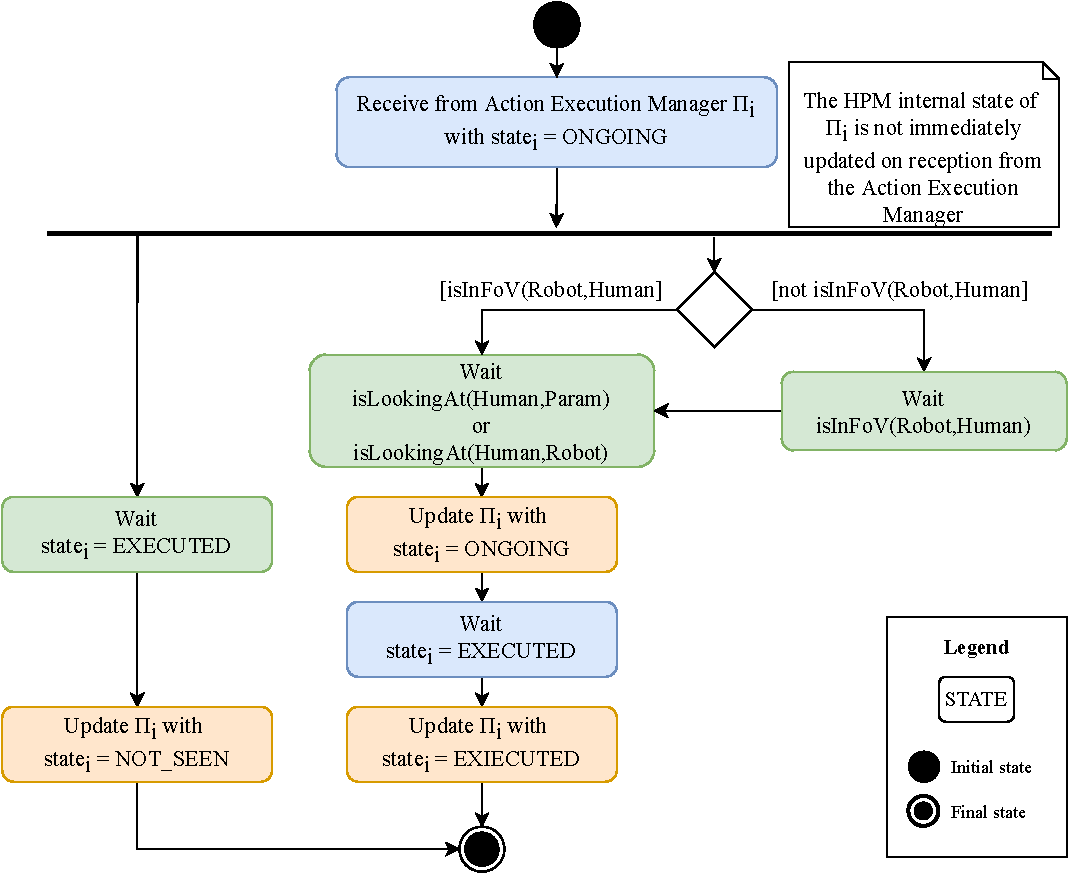
\includegraphics[width=\linewidth]{figures/chapter2/robot_action_hpm.pdf}
	\caption{Activity diagram representing what happens when the \acrfull{aem} sends to the \acrshort{hpm} that the robot started to execute an action. We represent in blue the nodes receiving data from the \acrshort{aem}, in green the ones receiving data from Ontologenius and in orange the ones updating the action state in the \acrshort{hpm} belief base.}
	\label{chap2:fig:robot_action_hpm}
\end{figure}

\clearpage

\subsection{Action Execution Management}\label{chap2:subsec:aem}

Deciding is not enough, the robot needs to be able to act. Thus, \acrshort{jahrvis} as an \acrfull{rja} called the \acrfull{aem}. It is composed of a generic part managing the general flow of an action execution, described in Algorithm~\ref{chap2:algo:exe_manage}, and of a task-specific part, specifying the distinctive characteristic of given actions which are instantiations of the \textsc{Execute} function in a separate ASL file, such as shown in Listing~\ref{chap2:lst:pick}. Moreover, all actions of the type PhysicalAction are realized based on action clients to communicate with the Motion Planner and Executor (see Figure~\ref{chap2:fig:archi}) which allows a fine management of the execution through feedbacks and error codes. For now, we do not treat specifically each error code. Finally, each instantiation of a PhysicalAction automatically starts and ends with the setting of the action parameters monitoring by the robot head, based on the head management presented in the next paragraph.

\begin{algorithm}[!htb]
	\caption{Action execution management}
	\label{chap2:algo:exe_manage}
	\begin{algorithmic}
	\Function{ExecuteAction}{primTask($i$,$name$,robot,$params$)}
	\If{$name \in$ PhysicalAction}
		\State \textsc{SendMessage}([\acrshort{rpm},\acrshort{hpm},\acrshort{ham}], primTask($i$,\algConst{ONGOING}))
	\ElsIf{$name \in$ CommunicateAction}
		\State \textsc{SendMessage}(CommManager, primTask($i$,\algConst{TODO}))\Comment{\algConst{ONGOING} state set \\\hfill by the \acrshort{cm}}
	\EndIf
	\State $action \coloneqq$ \textsc{ActionParsing($name$,$params$)}
	\State \textsc{Execute($action$)}
	\If{$name \in$ PhysicalAction}
		\State \textsc{SendMessage}([\acrshort{rpm},\acrshort{hpm},\acrshort{ham}], primTask($i$,\algConst{EXECUTED}))
	\ElsIf{$name \in$ CommunicateAction}
		\State \textsc{SendMessage}([\acrshort{rpm},\acrshort{hpm}], primTask($i$,\algConst{EXECUTED}))
	\EndIf
	\EndFunction
	\end{algorithmic}
\end{algorithm}	

\begin{lstlisting}[label={chap2:lst:pick},caption=Example of a PhysicalAction for execution by the Motion Planner and Executor.]
	@pick[atomic]
	+!pick(Params): true <-
			+planPick("armUsed", right_arm);
			planPick(Obj);
			execute("pick").
\end{lstlisting}

As for CommunicateAction, their parameters are reorganized and then the action is sent to the \acrshort{cm} for execution. An example is given in Listing~\ref{chap2:lst:comm_act}.

\begin{lstlisting}[label={chap2:lst:comm_act},caption=Example of a CommunicateAction for execution by the Communication Manager.]
	+!robot_tell_human_to_tidy(Params): true <-
			.nth(1, Params, Object);
			.nth(2, Params, Table);
			?action(ID,_,Name,_,Params);
			.send(communication,askOne,askActionsTodo(
				[action(ID,"PickAndPlaceAction",[Object,Table])],_),
				Answer).
\end{lstlisting}

\paragraph{Robot Resource Management}\label{chap2:para:resource_m}

The correct handling of the resources (head, arms, base...) of a robot is critical to perform a task, but it can be cumbersome for a deliberative component, such as \acrshort{jahrvis}, to do all the micro-management required. To tackle this issue, a physical resource management system has been designed by Guillaume Sarthou and Guilhem Buisan, inspired by Devin~\cite{devin_2017_decisional}. For each of the identified resources is instantiated a component called \emph{Resource Manager}, having two types of input: permanent channels, that can be preempted at any time (\eg look at the head of the human interacting with it) and finite state machines which are not preemptable (\eg set of commands to scan a table). A component called \emph{Resource Synchronizer} deals with actions requiring multiple resources such as the human-aware navigation which uses the head and the base. The synchronizer also reports the status of the ongoing coordination signal to \acrshort{jahrvis} to monitor the progress of the action. Finally, a priority scheme has been implemented to handle multiple active inputs at the same time for one resource. 

Such component allows \acrshort{jahrvis} to be agnostic about the used robotic platform, as it offers the same interface for whichever one. Moreover, it enables joint attention with a nice head control as \acrshort{jahrvis} can switch priorities between three types of permanent channels that have been defined, depending on where we are in the task: environment monitoring, human head monitoring and human hand monitoring. The two latter are set with the head and hand of the human the robot is interacting with as point to follow, whereas the environment monitoring channel receives new point of focus according to the needs of the task (\eg the cube the robot should pick or the box in which the human has to put an object). Thus, when the agents are talking together, \acrshort{jahrvis} will set the human's head with the highest priority, but when the robot has to pick a cube, it will be the environment monitoring that will have priority. Finally, the head behavior can be controlled not only based on visual inputs but also on laser inputs for example if it has some. Indeed, according to the task context, it can be interesting for the robot to know what is going on around it. It this case, a channel can be instantiated so the robot can react when it detects moves with its laser and then looks in this direction.

\subsection{Communication Management}\label{chap2:subsec:comm}
The last \acrshort{rja} involved in the robot decision and control is the \acrfull{cm}. It is not dedicated to complex talks with the human but to enable the robot to make and understand communication during collaborative tasks, because as shown in Section~\ref{chap1:subsec:comm}, it is important. This process is based on a software for Natural Language Processing (NLP) and closely linked to a domain-specific planner called \acrfull{reg}. This latter has been developed by Guillaume Sarthou and Guilhem Buisan~\cite{buisan_2020_efficient}. It aims, regarding the current symbolic state of the world, at finding the minimal set of relations to communicate and allow the listener to identify a given entity. For example, if the robot wants to talk about a given cube on a table but there are three of them, two (blue and red) on the table and one (blue) on a close furniture, how can it do? Well, it queries the \acrshort{reg} which answers with a nominal group such as ``the blue cube on the table''.


\paragraph{To  Issue Communications}
As shown above, three other processes, the \acrlong{ism}, the \acrlong{hpm} and \acrlong{aem}, can query the \acrshort{cm} to issue a communication to the human. We defined several types of communicative acts the robot can do:
\begin{inlineEnumerate}
	\item to do social chat for interaction session opening and closing (\eg ``hello''),
	\item to give information about its abilities/role (\eg ``I'm here to help you find your way''),
	\item to initiate a shared goal (\eg ``Let's do this package''),
	\item to give information about the ongoing task (\eg ``I cleaned the table''),\label{chap2:emum:comm1}
	\item to ask information about the ongoing task (\eg ``Have you cleaned the table?''),
	\item to request the human to perform an action (\eg ``Can you clean the table?''), and\label{chap2:emum:comm2}
	\item to give up the shared goal (\eg ``I'm sorry I give up, I'm failing'')
\end{inlineEnumerate}

We focused on the communicative acts described in \ref{chap2:emum:comm1} and \ref{chap2:emum:comm2} with the verbalization of actions presented in Algorithm~\ref{chap2:algo:action_verba}, developed in collaboration with Guillaume Sarthou. 

As the communication is important, it is important to minimize the risk that it gets lost. Thus, when the \acrshort{cm} receives a communication to perform from another \acrshort{rja}, it ensures that it perceives the human before issuing the communication so it has more chance to get the human's attention. Therefore, it sets the monitoring channel of the Robot Resource Manager on the human head monitoring (see Section~\ref{chap2:para:resource_m}).

Moreover, when the robot needs to communicate to the human that it has does a given action or to ask them to perform one, it needs to verbalize it properly. Still in the spirit of a generic system, the algorithm that we developed is not task or action specific. Action labels (presented in Section~\ref{chap2:subsubsec:action_rep} and verb conjugation (tense and persons) are stored in Ontologenius which can be manually fed with new ones when needed. Let's take an example with the robot informing the human it has performed a drop action called ``robot\_drop\_cube'' in the plan, with ``cube\_1'' and ``green\_box'' as parameters. First, the \acrshort{cm} queries Ontologenius to get the closest class in the hierarchy with labels. Here, it is ``DropAction''. There are three possible labels for this action, so the robot has the possibility to communicate about it with different action parameters: [{Agent} @Drop {Cube}, {Agent} @Drop in {Container}, {Agent} @Drop {Cube} in {Container}]. Thus, the \acrshort{cm} finds which label matches its parameters, based on the parameter number and on their class. Then, in our case, this is ``{Agent} @Drop {Cube} in {Container}]''. Next, for each parameter, it tries to find the right verbalization, either it will be a Referring Expression or the parameter label stored in Ontologenius, and replace them in the class action label. So, we would have something like ``{Agent} @Drop the blue cube on the table in the box''. Finally, it replaces ``{Agent}'' with the action actor and ``@Drop'' with the right conjugation. As the \acrshort{cm} wants to refer to an action the robot has done, it queries the Ontology with the conjugation of ``Drop'' at the past first singular person, which is ``dropped''. Then, the result of the action verbalization is ``I dropped the blue cube on the table in the box''. 

When the \acrshort{cm} wants to ask the human to perform an action, it uses the same algorithm and turn the sentence into an interrogative form with the verb ``can''. As \acrshort{jahrvis} manipulates conditional plans, the \acrshort{cm} can take as input list of actions and separate them with ``or'' when communicating about them. And, when it wants to communicate about the human having to perform several actions in a row, it using ``and''.
 
\begin{algorithm}[!htb]
	\caption{Action verbalization}
	\label{chap2:algo:action_verba}
	\begin{algorithmic}
	\Function{ActionVerbalization}{$agent$,$action$,$parameters$,$tense$}
	\State $labelList \coloneqq$\textsc{GetClassActionLabels($action$)}\Comment{Query to Ontologenius}
	\State $actionVerba \coloneqq$\textsc{LabelToWords}($labelList$,$parameters$)
	\If{$agent \in$ robot}
		\State $person \coloneqq$ FirstSingularPersonalForm
		\State $pronoun \coloneqq$ I
	\ElsIf{$agent \in$ human}
		\State $person \coloneqq$ SecondSingularPersonalForm
		\State $pronoun \coloneqq$ you
	\EndIf
	\State $verb \coloneqq$\textsc{GetVerb}($actionVerba$)
	\State $conjugatedVerb \coloneqq$\textsc{GetConjug}($actionVerba$,$verb$,$person$,$tense$)\Comment{Query to \\\hfill Ontologenius}
	\State $actionVerba \coloneqq actionVerba.$\textsc{Replace}("\{Agent\}",$pronoun$)
	\State $actionVerba \coloneqq actionVerba.$\textsc{Replace}("@$verb$",$conjugatedVerb$)
	\EndFunction
	\Statex
	\Function{LabelToWords}{$labelList$,$parameters$}
	\State $actionVerba \coloneqq$""
	\ForEach{$label$}{$labelList$}
		\State $labelClassParams \coloneqq$\textsc{RegexMatch}("\{(?!Agent)(.*?)\}",$label$)
		\If{\textsc{Length}($labelClassParams$)=\textsc{Length}($parameters$)}
		\ForEach{$param$}{$parameters$}
			\ForEach{$labelClassParam$}{$labelClassParams$}
			\If{$param \in labelClassParam$} \Comment{Query to Ontologenius}
				\If{$actionVerba=$""}
					\State $actionVerba \coloneqq label$
				\EndIf
				\If{$param \in$ Pickable and \fact{isAbove}{$param$}{Support}}
					\State $param \coloneqq$\textsc{GetReferringExpression($param$)}
				\Else
					\State $paramVerba \coloneqq$ \textsc{GetParamVerba($param$)}\Comment{Query to \\\hfill Ontologenius}
				\EndIf
				\State $actionVerba \coloneqq actionVerba.$\textsc{Replace}("\{$labelClassParam$\}",$paramVerba$)
				\State \textbf{break}
			\EndIf
			\EndFor
		\EndFor
		\EndIf
	\EndFor
	\EndFunction
	\end{algorithmic}
\end{algorithm}	
	


\paragraph{To Understand Communications}
That the robot communicates to the human is important but that it would be able to receive communication from them is as well. The human should be allow to communicate about the plan such as to ask precision about a given action, to signal that something is not going well or to ask the robot to perform an action. We focused on the latter in collaboration with Guillaume Sarthou. 

The Algorithm~\ref{chap2:algo:human_instruction} allows the \acrshort{cm} to translate a human instruction to give an action (with one parameter) to perform to the robot into an instruction understandable by the \acrlong{aem}. When the \acrshort{cm} receives a human sentence such as ``Take the blue cube'', it queries the \acrfull{nlp} component which returns the action name it isolated from the rest of the sentence, a \sparql query corresponding to the parameter and a comprehension score. Then, it requests Ontologenius for the list of objects corresponding to the \sparql query, from the human's perspective. Indeed, the robot could see a blue cube which is not visible by the human, it this case, it will not be part of the returned objects as it is not part of the human's knowledge. If the human has properly given their instruction, the list size should be 1 and the algorithm is over. However, for some reason, they made have been imprecise. For example, there might be two blue cubes on the table. In this case, the \acrshort{cm} gets from Ontologenius the \sparql query corresponding to each object, with elements allowing to discriminate between them. Then, it requests the \acrshort{reg} for the verbalization of these objects, based on their \sparql description. Thus, we could have the \acrshort{cm} to ask the human something like ``Do you mean the blue cube on the table or on the shelf?''. Finally the function starts over with the human answer which could be ``the blue cube on the table'' -- the \acrshort{cm} keeps the action of the initial instruction into memory.

Finally, once the \acrshort{cm} isolated an action and a parameter, it sends them to the \acrlong{aem}.

\begin{algorithm}[!htb]
	\caption{Understanding of a human instruction}
	\label{chap2:algo:human_instruction}
	\begin{algorithmic}
	\Function{GetActionToPerform}{$sentence$,$context$}
	\State $\langle act, sparqlQ, score \rangle \coloneqq$ \textsc{GetSentenceSegmentation($sentence$)} \Comment{Query \\\hfill to REG}
	\If{$score > Score_{min}$}
		\State $merged \coloneqq$\textsc{MergeSparqlWithContext}($sparqlQ,context$)\Comment{Query \\\hfill to REG}
		\State $matchingObjects \coloneqq$ \textsc{SparqlToObjects}($merged$)\Comment{Query \\\hfill to Ontologenius}
		\If{\textsc{Length}($matchingObjects$)=1}
			\State \Return $act,matchingObjects[0]$
		\Else
			\State $question \coloneqq$``do you mean ''
			\ForEach{$object$}{$matchingObjects$}
				\State $sparqlO \coloneqq$\textsc{GetSparql($object$)}\Comment{Query to Ontologenius}
				\State $objectVerba \coloneqq$\textsc{GetObjectVerbalization($sparqlO$)}\Comment{Query \\\hfill to REG}
				\State $question \coloneqq question + objectVerba$
			\EndFor
			\State $answer \coloneqq$\textsc{AskHuman}($question$)
			\State \textsc{AnalyzeSentence}($answer$,$merged$)
		\EndIf
	\EndIf
	\EndFunction
	\end{algorithmic}
\end{algorithm}		


\clearpage
\subsection{Conclusion and Future work}
In this chapter, we have proposed a generic supervision component providing robot decision and control to the robotic architecture it is integrated to, for collaborative robots. The developed \acrfull{rja} have their basis into the joint action principles presented in Chapter~\ref{chapter:chap1}. It endows the robot with knowledge representation, perspective-taking and \acrshort{tom}, joint attention, monitoring, communication, shared plan management.  


We had a lot of ideas but implemented only a few of them. To build a supervision system to endow a robot with autonomy when performing collaborative tasks with a human is not an easy thing, especially when thinking to genericness and re-usability. The work presented in this chapter provides a basis for an even more complex system, handling contingencies, and with a more refined interaction session manager which could integrate a nice goal negotiation component. Moreover, once the robot performs quite well with one task and one human, why not add other humans and/or other tasks in parallel?

%limit : use of shared plans as these ones. what should be interesting would be to have plans with actions having conditions about what should be executed before it and not predecessors

In Section~\ref{chap2:sec:control}, we presented the \acrshort{jahrvis} processes for decision-making and robot control. Chapter~\ref{chapter:chap3}, n the context of a direction-giving task, will feature the \acrlong{ism}, an early version of the \acrlong{rpm} and the \acrlong{aem}. Chapter~\ref{chapter:chap4}, as for it, will emphasize the \acrlong{rpm}, the \acrlong{hpm}, the \acrlong{aem}, the \acrlong{ham} and the \acrlong{cm}.

\ifdefined\included
\else
\bibliographystyle{acm}
\bibliography{These}
\end{document}
\fi
